\documentclass[12pt]{article}
\usepackage{verbatimbox}
\usepackage{lipsum}
\usepackage{shortvrb} 
 \usepackage[T1]{fontenc}
\usepackage[utf8]{inputenc}
\usepackage{pmboxdraw}
\usepackage{newunicodechar}

\usepackage[hidelinks]{hyperref}
\usepackage[margin=1.1in ,left = 1.20in ,includefoot]{geometry}
\usepackage{graphicx}
\usepackage{float}
\usepackage[]{algorithm2e}
\usepackage{epstopdf}
\usepackage[toc,page]{appendix} 
\usepackage{amsmath}
\usepackage{fancyhdr}
\usepackage{moreverb}
\pagestyle{fancy}

%\pagestyle{headings}
\rhead{}

\usepackage{enumitem}
\usepackage{gensymb}
\usepackage{nth}
 \usepackage{hyperref}
\usepackage{subfig}
\usepackage[hidelinks]{hyperref}
\setlength{\footskip}{.8in}


\usepackage{afterpage}

\newcommand\blankpage{%
	\null
	\thispagestyle{empty}%
	\addtocounter{page}{-1}%
	\newpage}


% Default fixed font does not support bold face
\DeclareFixedFont{\ttb}{T1}{txtt}{bx}{n}{12} % for bold
\DeclareFixedFont{\ttm}{T1}{txtt}{m}{n}{12}  % for normal

% Custom colors
\usepackage{color}
\definecolor{deepblue}{rgb}{0,0,0.5}
\definecolor{deepred}{rgb}{0.6,0,0}
\definecolor{deepgreen}{rgb}{0,0.5,0}

\usepackage{listings}

% Python style for highlighting
\newcommand\pythonstyle{\lstset{
language=Python,
basicstyle=\ttm,
otherkeywords={self},             % Add keywords here
keywordstyle=\ttb\color{deepblue},
emph={MyClass,__init__},          % Custom highlighting
emphstyle=\ttb\color{deepred},    % Custom highlighting style
stringstyle=\color{deepgreen},
frame=tb,                         % Any extra options here
showstringspaces=false            % 
}}


% Python environment
\lstnewenvironment{python}[1][]
{
\pythonstyle
\lstset{#1}
}
{}

% Python for external files
\newcommand\pythonexternal[2][]{{
\pythonstyle
\lstinputlisting[#1]{#2}}}

% Python for inline
\newcommand\pythoninline[1]{{\pythonstyle\lstinline!#1!}}











\begin{document}
 
\begin{titlepage}
	
\thispagestyle{empty}

\begin{center}
\large {A project report on}

\Huge{\bfseries Indoor Navigation and Localization Mobile Robot }\\[0.5cm]
\large{(Final year project)}
 \\
 Submitted in partial fulfillment of the requirement for the award of the\\
 \large {Degree of Bachelor in }\\
 
 \large{\bfseries COMPUTER AND SYSTEMS ENGINEERING }\\
 
 \vspace{1.2cm}
 \begin{figure}[H]
\centering

\includegraphics[width =.45\textwidth]{Fig/faculty.png}

\end{figure}
 \vspace{.5cm}
\end{center}
 
\hspace{1cm} {\LARGE \bfseries Submitted by}  \hspace{3.5cm} {\LARGE \bfseries Supervised by:}


\hspace{0.5cm} {\bfseries  Ahmed Abdelbadee Elsayed}\hspace{2.5cm} {\bfseries  Dr.Ahmed Mohamed Helmi }

\hspace{0.5cm} {\bfseries Ahmed Abdelbasit Mohamed} 


\hspace{0.5cm} {\bfseries  Aya Ibrahim Elsayed} 


\hspace{0.5cm} {\bfseries Nourhan Mansour Mohamed} 


\hspace{0.5cm} {\bfseries Omar Raafat Abdullatif}

 
\hspace{0.5cm} {\bfseries  Yasmin Ahmed Abdelbasit}

 


\begin{center}
\today \\
 
 {\Large  \bfseries   Faculty of Engineering }\\
 
{\LARGE \bfseries Zagazig University } 
\end{center}



% Bottom of the page
 
 
 
 
 
 
 \afterpage{\blankpage}

\renewcommand{\headrulewidth}{0pt}

\end {titlepage}






\pagenumbering{roman}
\section*{\begin{center}
Abstract
\end{center}}

	This project introduces a small-size mobile robot to be used for indoor navigation. It can be operated either autonomously or controlled by man remotely over the network. Its size make it able to navigate in small places and narrow paths man can not go through.\\
	Man can discover the environment around it via a video stream transmitted by a camera free to rotate right, left, up and down. A user-friendly controller box is provided for manned control to guide robot's motion, set camera orientation and switch on/off flash light.\\
	The autonomous navigation is based on graph theory and artificial intelligence search algorithms in a predefined map for the environment around robot. With the help of Landmarks detection by computer vision, the robot can identify its location periodically on his path from source to destination. This provides a great help to avoid accumulated errors caused by hardware or sensors in accuracy.\\
	A computer graphical user interface (GUI) application is developed to easily reach the functionality of robot. By this application one can select either autonomous or manual mode and deal with each mode utilities.\\
	The project is based on Robots Operating System (ROS) which makes its functionality reusable in other projects. Modularity and readable codes are considered in the design and implementation of software nodes. Also an optimized communication protocol is developed among project's parts.\\
	About future work there is a wide field of updates like object detection, On-line Mapping of new Environments and installation of manipulator (i.e. robot arm) for a variety of	tasks.

 
\addcontentsline{toc}{section}{\numberline{}Abstract}

\afterpage{\blankpage}
\newpage


\section*{\begin{Large}
		Acknowledgments
\end{Large}}

\noindent We want to thank our department, computer and systems dept. at Zagazig University, who provided valuable comments, ideas, and assistance, which were essential to this study. This work is developed for and fully funded by Zagazig University, Faculty of Engineering as a part of development for a robotic platform.\\

\noindent First of all, We want to thank our supervisor Dr.Eng. Ahmed Helmi for giving us the chance to work on this project and helped us to participate in a lot of conferences and competitions. Also we want to thank him for his valuable notes and advices for developing the proposed algorithm applied in our project.\\

\noindent We also want to thank Dr.Ing Mohamed Nour for his helpful guidance and opening the way to learn and deal with Robots Operating System platform which represents the main core of our project.\\

\noindent We would like to thank our friends for helping us in the manufacturing process of the robot frame. And many thanks to Eng. Mahmoud Ibrahim for providing us the material of the robot frame which makes our project more robust and leads to better performance.\\

\noindent We would like to thank our parents and family for giving us the encouragement to reach our goals and saved no effort to provide us all the needs.


\addcontentsline{toc}{section}{\numberline{}Acknoledgements}

\afterpage{\blankpage}

\newpage


\tableofcontents
\afterpage{\blankpage}
\newpage

\renewcommand{\headrulewidth}{0pt}
\section*{\begin{Large}
		Key abbreviations
\end{Large}}

\begin{tabular}{  l    l   }
	ROS & Robots Operating System	\\
	GUI & Graphical User Interface	\\
	RPi &   Raspberry Pi	\\
	NiMH & Nickel–Metal Hydride\\
	BMP & Bitmap \\
	GBFS & Greedy Best First Search\\
	PPR & Pulse Per Revolution \\
	IR & Infra Red \\
	SSH & Secure Shell\\
	IDE & Integrated Development Environment\\
	
	PID & Proportion Integral Derivative  \\  
	PWM &  Pulse Width Modulation  \\   
	$I^2C$  & Inter-Integrated Circuit   \\  
	IMU &  Inertial Measurement Unit \\  
	LiPo &   Lithium Polymer\\ 
	RPM   & Revolution Per Minute  \\
	ADC   & Analog-Digital Converter   \\  
	LPF & Low Pass Filter \\
	FPS & Frame Per Seconds\\
	GND & Ground
	
\end{tabular} 

\addcontentsline{toc}{section}{\numberline{}Key abbreviations}



\newpage

\renewcommand{\headrulewidth}{.5pt}

\listoffigures
\thispagestyle{empty}
\newpage
\pagenumbering{arabic}
\setcounter{page}{1}


\section{Introduction}
 In daily life there are a lot of situations in which robots are needed to perform some tasks man can not deal with. Some of these situations may be risky, difficult or such impossible for man to do. Think about a risky place we want to discover like disasters area, places of extreme environmental conditions or military purposes. In these situations introducing a robot is important for saving human life.\\
 Robots also can help people of special needs with what they can not do like carrying heavy things, holding and placing parts or even home cleaning.\\
 Robots have many configurations, styles and mechanisms for motion. Some are legged, others are wheeled and the rest can fly, swim or dive. Each configuration has its functionality that others can not do and also has limitations.
 In our project we introduce a robot with good navigation and localization technique to solve a lot of problems mentioned above in this section. 

\begin{figure}[h]
\centering
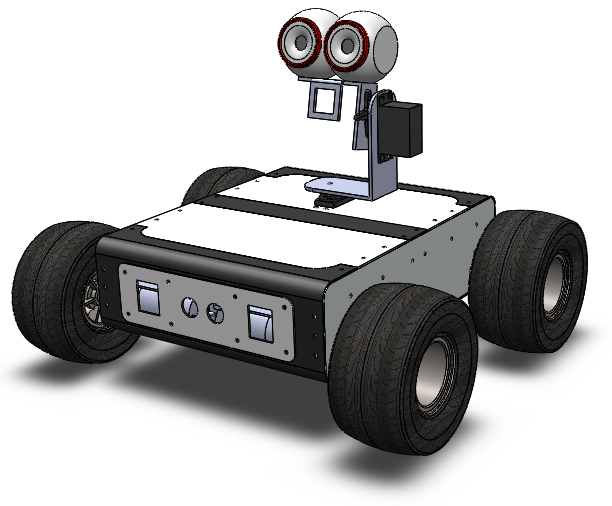
\includegraphics[width =.4\textwidth]{Fig/Introduction.png}
\caption{ A 3-D model for robot frame}
\end{figure}

%\clearpage

\subsection{History of Mobile Robots} 
Mobile robots have the capability to move around in their environment and are not fixed to one physical location. Mobile robots can be "autonomous" (AMR - autonomous mobile robot) which means they are capable of navigating an uncontrolled environment without the need for physical or electro-mechanical guidance devices. Alternatively, mobile robots can rely on guidance devices that allow them to travel a pre-defined navigation route in relatively controlled space (AGV - autonomous guided vehicle). By contrast, industrial robots are usually more-or-less stationary, consisting of a jointed arm (multi-linked manipulator) and gripper assembly (or end effector), attached to a fixed surface.\\
Mobile robots have become more commonplace in commercial and industrial settings. Hospitals have been using autonomous mobile robots to move materials for many years. Warehouses have installed mobile robotic systems to efficiently move materials from stocking shelves to order fulfillment zones. Mobile robots are also a major focus of current research and almost every major university has one or more labs that focus on mobile robot research. Mobile robots are also found in industrial, military and security settings. Domestic robots are consumer products, including entertainment robots and those that perform certain household tasks such as vacuuming or gardening. \cite{202}


\begin{figure}[H]
 \centering
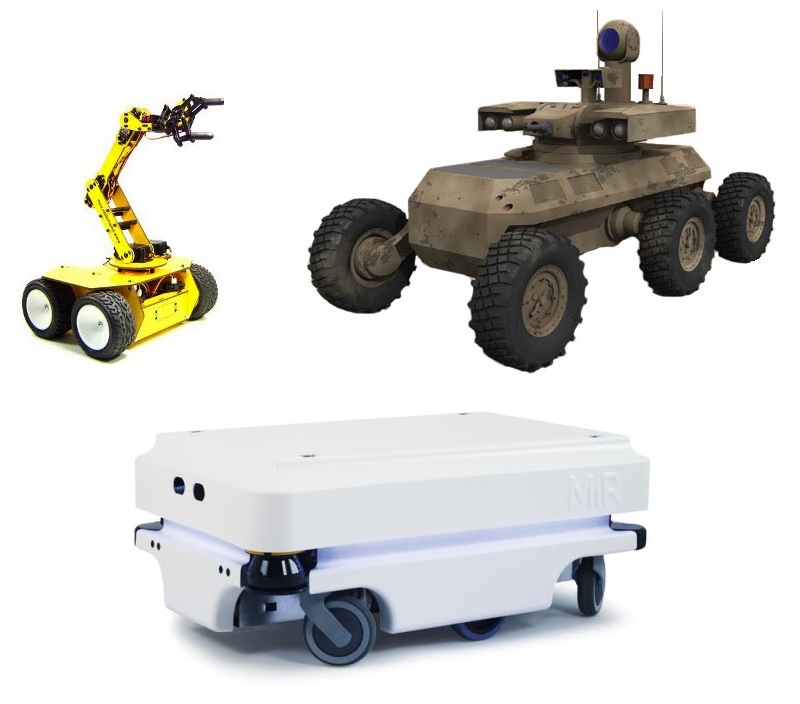
\includegraphics[width =0.6\textwidth]{Fig/mobile_robots_apps.jpg}
\caption{Different applications for mobile robots; industrial, military and transport}

\end{figure}

\subsection{Project Objectives}
The main objective of this project is to demonstrate a robust mobile robot in a small scale to perform an autonomous navigation from point to another. Also it is required for the robot to localize itself when asked to do. Both navigation and localization depends on the ability of robot to detect and recognize texts on landmarks that uniquely identifies specific nodes in the map.
For new environments whose map is not known, the robot can be guided remotely over the network to explore that location and a camera is provided for both steaming live video for the site around robot and to perform the computer vision task.
In the hardware level a robust controller is required to perform motion instructions with acceptable precision.

\newpage

\subsection{Limitations}
During our work we faced a lot of problems associated mostly with sensors. As we the main part in any control system is the feedback. This is because if we got a wrong indication for current state of system, we will perform a wrong reaction and the error increases more and more. In our project we need sensors to get information about the robot like position, velocity and orientation. Any missing part of them leads to both wrong estimation of state and wrong controller action.
In next sections we will talk about our trials, results and algorithms implemented to get the advantage of each sensor and avoid its misleading data.
\noindent But lets start from a high-level point of view and gradually take important topics with some details.

\subsection{Overview on the project parts}
The main system structure of our project as shown in figure \ref{fig:system-structure} consists of a GUI and controller box at user side and the master unit (RPi) at robot side. The operation starts from GUI to select the function needed and then a flow of communication commands are passed to master unit over the network to perform the required task. Controller box is used in manned mode of operation to guide robot motion and camera orientation. In next chapter we talk about the GUI; how you can use, how it is implemented and a quick over view on ROS (Robots Operating System).
\begin{figure}[H]
	\centering
	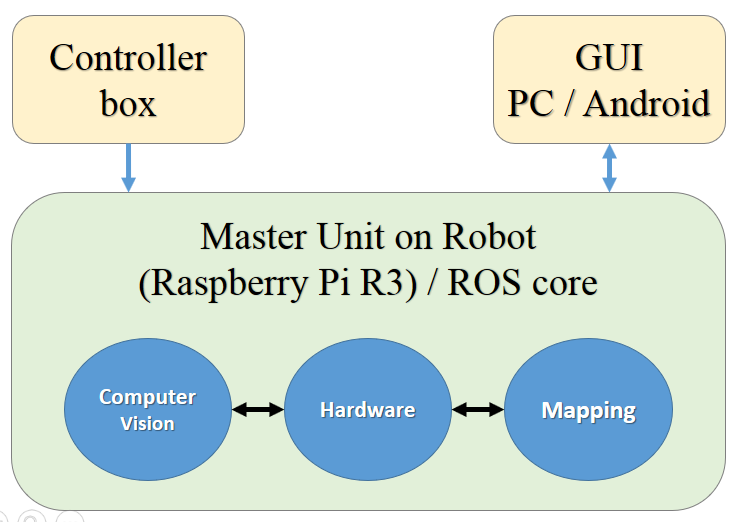
\includegraphics[width =0.6\textwidth]{Fig/overview.png}
	\caption{Clustered view of main system structure}
	\label{fig:system-structure}
\end{figure}
\newpage

\section{User Manual and GUI}
talk about how to use the GUI to run the project on different modes.

\newpage

\section{System Structure and Proposed Algorithm}
In the design stage of project, three main parts arises to be implemented; mapping, computer vision and hardware. Each part represents an executable program that can interact with other parts in a manner to fulfill the required task. So, lets first talk briefly about ROS and how it provided a great help in connecting project parts and how communication between processes becomes easy.



\subsection{Robots Operating System (ROS)}
The Robot Operating System (ROS) is a flexible framework for writing robot software. It is a collection of tools, libraries, and conventions that aim to simplify the task of creating complex and robust robot behavior across a wide variety of robotic platforms. \cite{201} \\
In ROS, Node is a common word that represents the executable file. So, in our project we have three main nodes; mapping, computer vision and hardware nodes. communication between nodes in ROS can be performed in many ways. The method we worked with is the message communication. Message represents the ROS data type. We developed a special type that can handle all communication needs between nodes. It is called Instruction and consists of a string variable that holds the command name and two float arguments. \\
Nodes can deal with messages in two manners; as a publisher, subscriber or both. Another word commonly used in ROS is the topic. It is considered as an intermediate program that holds any published message and forward it to all nodes that subscribed for it. This feature is very useful as a node can perform just one publishing command and any number of nodes can receive it. 
Now we know a bit about how ROS works and for more details and tutorials you can visit ROS tutorials site: http://wiki.ros.org/ROS/Tutorials. \\ \\
In next section we are to talk about our project nodes and how communication performed among them.
\begin{figure}[H]
	\centering
	
\includegraphics[width = 0.3\textwidth]{Fig/rosLogo.png}
	\caption{ROS logo.}
\end{figure}

\newpage

\subsection{Project Nodes and Communication Process}
As mentioned before, we have three main nodes; mapping, computer vision and hardware. the communication between them were created as shown in figure \ref{fig:nodes}. 
\begin{figure}[H]
	\centering
	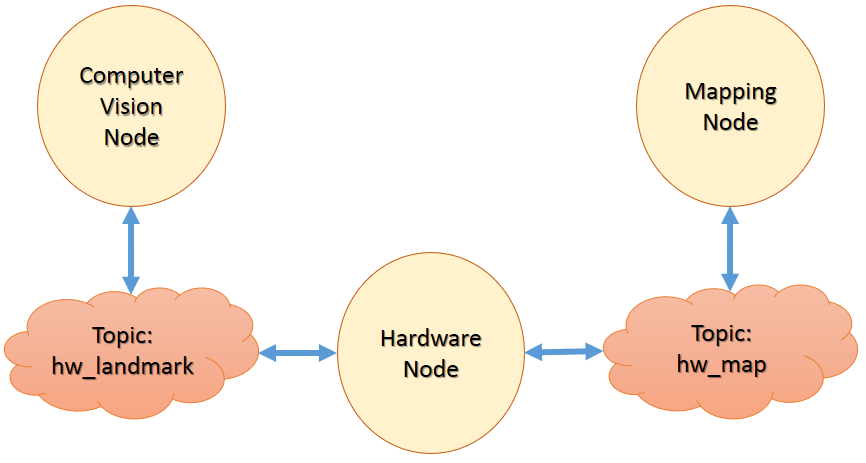
\includegraphics[width =0.6\textwidth]{Fig/Project-Nodes.png}
	\caption{The implemented nodes and advertised topics between them.}
	\label{fig:nodes}
\end{figure}
\noindent There are two advertised topics; hw\_landmark that connects hardware with computer vision and hw\_map that connects hardware to mapping node. Over the hw\_map topic the mapping node publishes the instructions that guide the robot from a landmark to another. When the robot reaches a new landmark, a tuning loop starts between hardware and computer vision node to put the robot exactly in front of the landmark. In this way, errors caused by inaccuracy of sensors or hardware motion performance are eliminated periodically resulting in a good autonomous navigation of the robot.\\
In next section we are to talk about the navigation algorithm and the sequence of instructions with some details.  




\subsection{Proposed Algorithm for Autonomous Navigation}
In the autonomous navigation mission, each of the three nodes has its own task to do. We can categorize these tasks in two phases. First phase is executed between Mapping and hardware node. Its goal is to guide the robot from one landmark to the next one on path to destination. Once the robot reaches that landmark or someplace near it, the second phase starts between computer vision node and hardware telling the robot how to move to stand exactly in front of the landmark. Figure \ref{fig:algorithm-phases} visualize these phases with brief description.

\begin{figure}
	\centering
	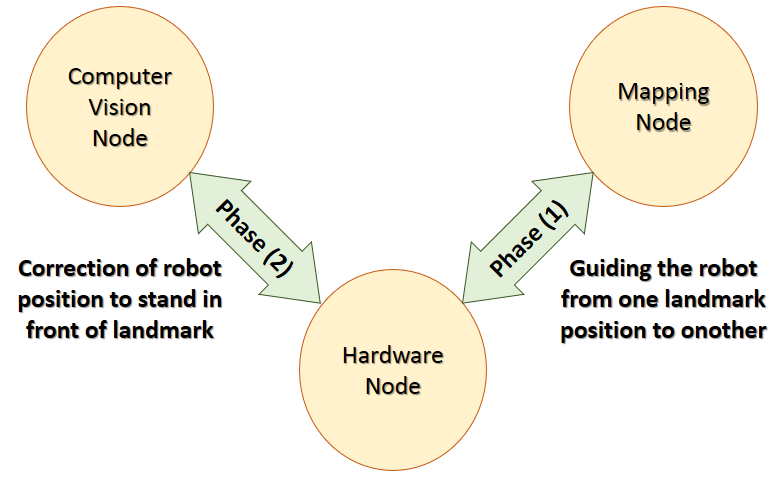
\includegraphics[width=0.7\textwidth]{Fig/Algorithm-phases.png}
	\caption{Proposed algorithm's phases}
	\label{fig:algorithm-phases}
\end{figure}

\noindent In the first phase, a sequence on instructions are passed from mapping to hardware node. These instructions can be 'move', 'rotate', 'rotate-camera' or a query for information of sensors. After each instruction the hardware responds by 'next\_step' command as an acknowledgment to mapping node that the last instruction is done. When the mapping node receives acknowledgment of last instruction, it sends a 'tune' command telling the robot to start the second phase. 

\noindent Second phase is a tuning process to eliminate any accumulated errors caused by hardware while performing mapping instructions. The computer vision node tries to guide the hardware to move in a way such that the land mark is detected at the center of picture frame. In this case, by knowing the distance between robot and wall we fully identify the robot position. Figure \ref{fig:localization} shows how localization is done by computer vision and range finder sensor.
\begin{figure}[H]
	\centering
	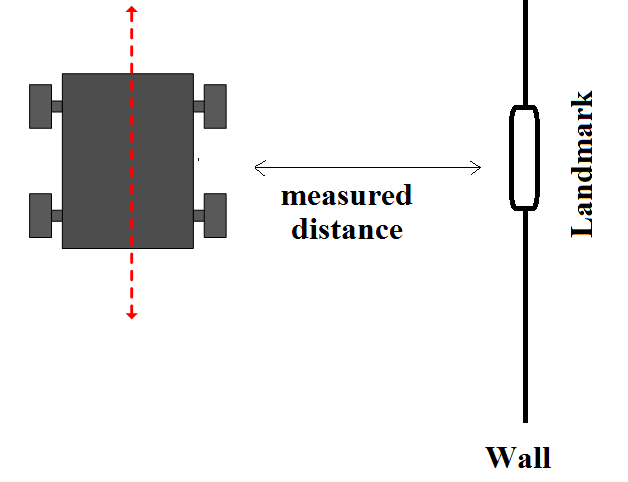
\includegraphics[width =0.4\textwidth]{Fig/localization.png}
	\caption{Localization using computer vision}
	\label{fig:localization}
\end{figure}

\noindent The flowchart of autonomous navigation process is provided ni figure \ref{fig:full-algorithm} showing the whole communication steps and conditions involved in such process. You can identify in this flowchart the role of each node and how it deals with others.

\newpage

\begin{figure}
	\centering
	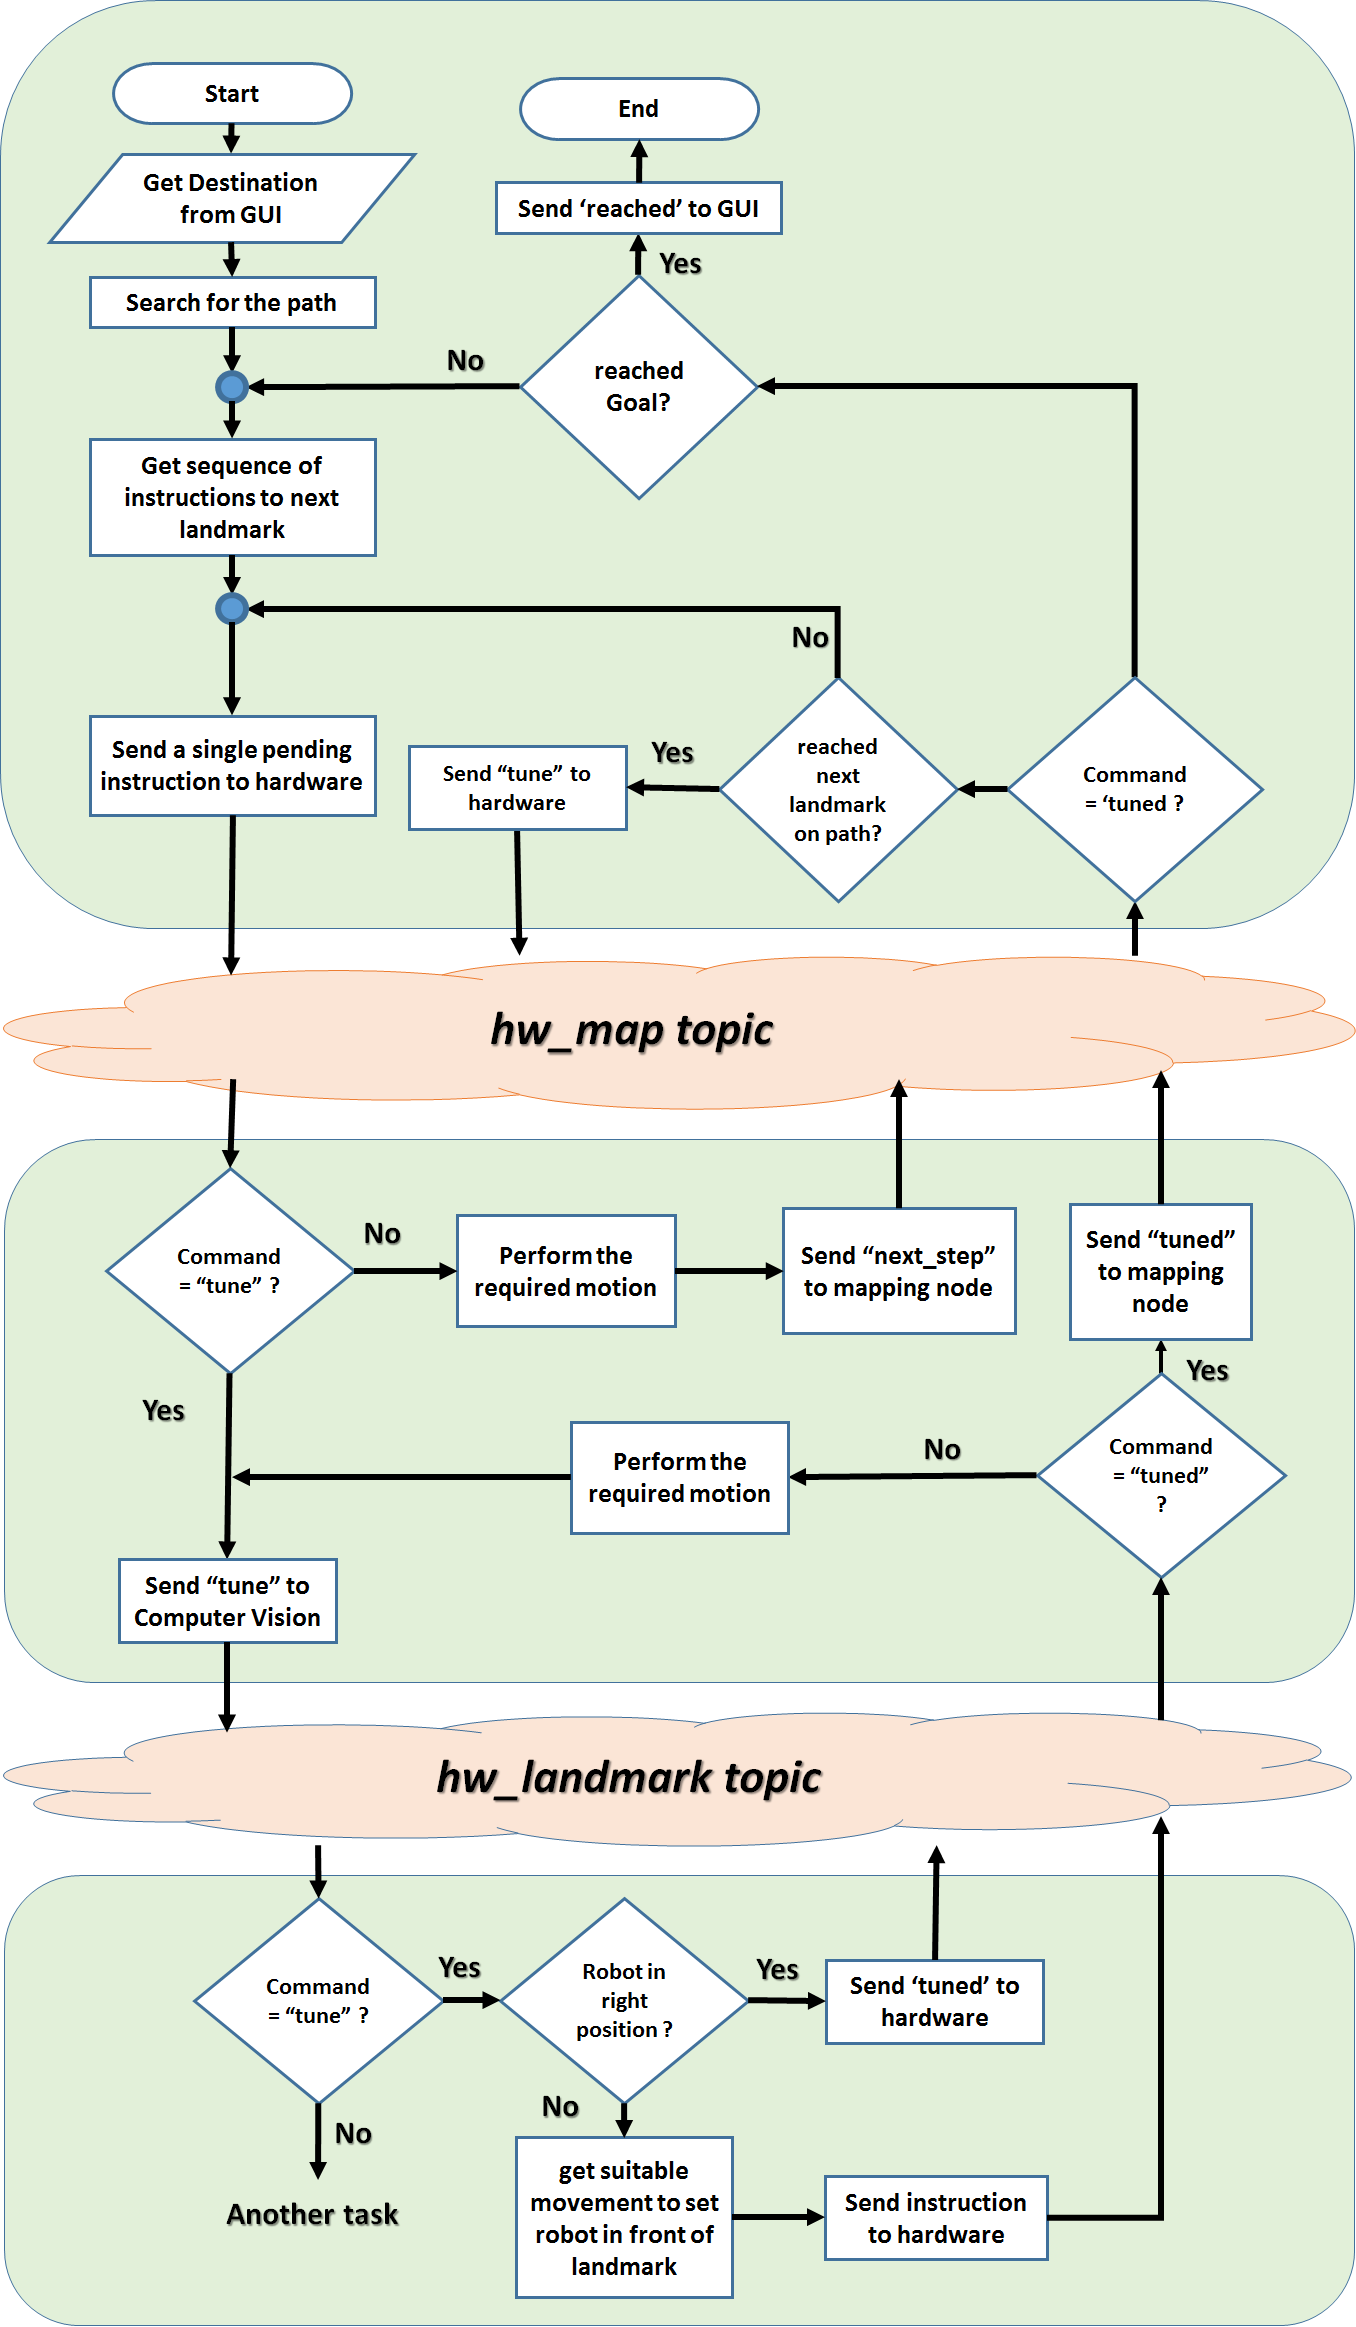
\includegraphics[width =0.75\textwidth]{Fig/full-algorithm.png}
	\caption{Flowchart for whole algorithm applied for autonomous navigation.}
	\label{fig:full-algorithm}
\end{figure}

\newpage
\clearpage
\newpage

\section{GUI Implementation}
talk about the Java application and how it is implemented, how it communicates with master unit to send navigation instruction. also how video stream is received

\newpage

\section{Mapping of Environment}
Our robot is an off-line mapping system , meaning it only moves in a region when it has a map for it stored in its memory , we store the map in BMP format and the location of landmarks in a TXT file , and the mapping part gives the hardware part the instructions necessary to navigate from a start landmark to a destination landmark

\subsection{Introduction}
In this work, we present an algorithm for path planning to a target for mobile robot in known environment. The proposed algorithm allows a mobile robot to navigate through static obstacles, and finding the path in order to reach the target without collision. This algorithm provides robot the ability to move from the initial position to the final position (target). The path finding strategy is designed using a greedy and A* algorithms. The robot moves within the environment by sensing and avoiding the obstacles coming across its way towards the target. When the mission is executed, it is necessary to plan an optimal or feasible path for itself avoiding obstructions in its way and minimizing a cost such as time, energy, and distance. The proposed path planning must make the robot able to achieve these tasks: to avoid obstacles, and to make ones way toward its target. 

\subsection{Mapping Algorithms considered}
Navigating a terrain and finding the shortest path to a Goal location is one of the fundamental problems in path planning. While there are many approaches to this problem, Our robot uses an off-line map to navigate through its environment , so it needs a search algorithm to find the best way to reach the destination node from a start one. We had two algorithms to consider , GBFS and A*.

\subsubsection{Greedy Best First Search(GBFS) Algorithm :}
This algorithm depends on a heuristic function which is the direct distance from the node to the goal node , and traverses its graph by selecting the node with the lowest heuristic in its frontier.

\begin{itemize}
	\item \textbf{Advantages:}
		\begin{itemize}
			\item Fast(less than a second) , which allows for remapping and obstacle avoidance
			\item Consumes the least possible memory space
			
		\end{itemize}
	\item \textbf{Disadvantages:}
		\begin{itemize}
			\item It does not give the optimal route from source to destination
			\item Not guaranteed to find the goal
			
		\end{itemize}
\end{itemize}

\subsubsection{A* Algorithm:}
This algorithm depends on both a heuristic function (which is still the direct distance from the node to the goal node) and the cost which is the number of nodes that led to this node , and traverses its graph by selecting the node with the lowest sum of them in its .

\begin{itemize}
	\item \textbf{Advantages:}
	\begin{itemize}
		\item Balance between space-time consumption and accuracy
		\item Guaranteed to find the goal
		\item Gives the best possible path from start point to goal
		
		
	\end{itemize}
	\item \textbf{Disadvantages:}
	\begin{itemize}
		\item Slower than acceptable for real time (A few seconds)
		
	\end{itemize}
\end{itemize}

\subsubsection{Algorithm used in our project}
After some tries and results demonstration We used a merge between them , good , but how?\\
We used a map with the path we want the robot to follow when possible is white and all others are grey (127 of 255 brightness) , the algorithm uses heuristic only in white areas (GBFS) and the sum of heuristic and cost in gray areas (A*) , this way , we ensure the algorithm moves in the wanted path unless necessary , we also used lines with (195 of 255) gray to indicate whether the robot is next to a landmark or not .
We also noticed that the GBFS algorithm doesn’t give the same results when going from source to destination and vice-versa , so we made the code run the algorithm both ways and choose the best to be operated.
Flowchart of whole mapping role is shown in figure \ref{fig:map-flowchart}.

\begin{figure}
	\centering
	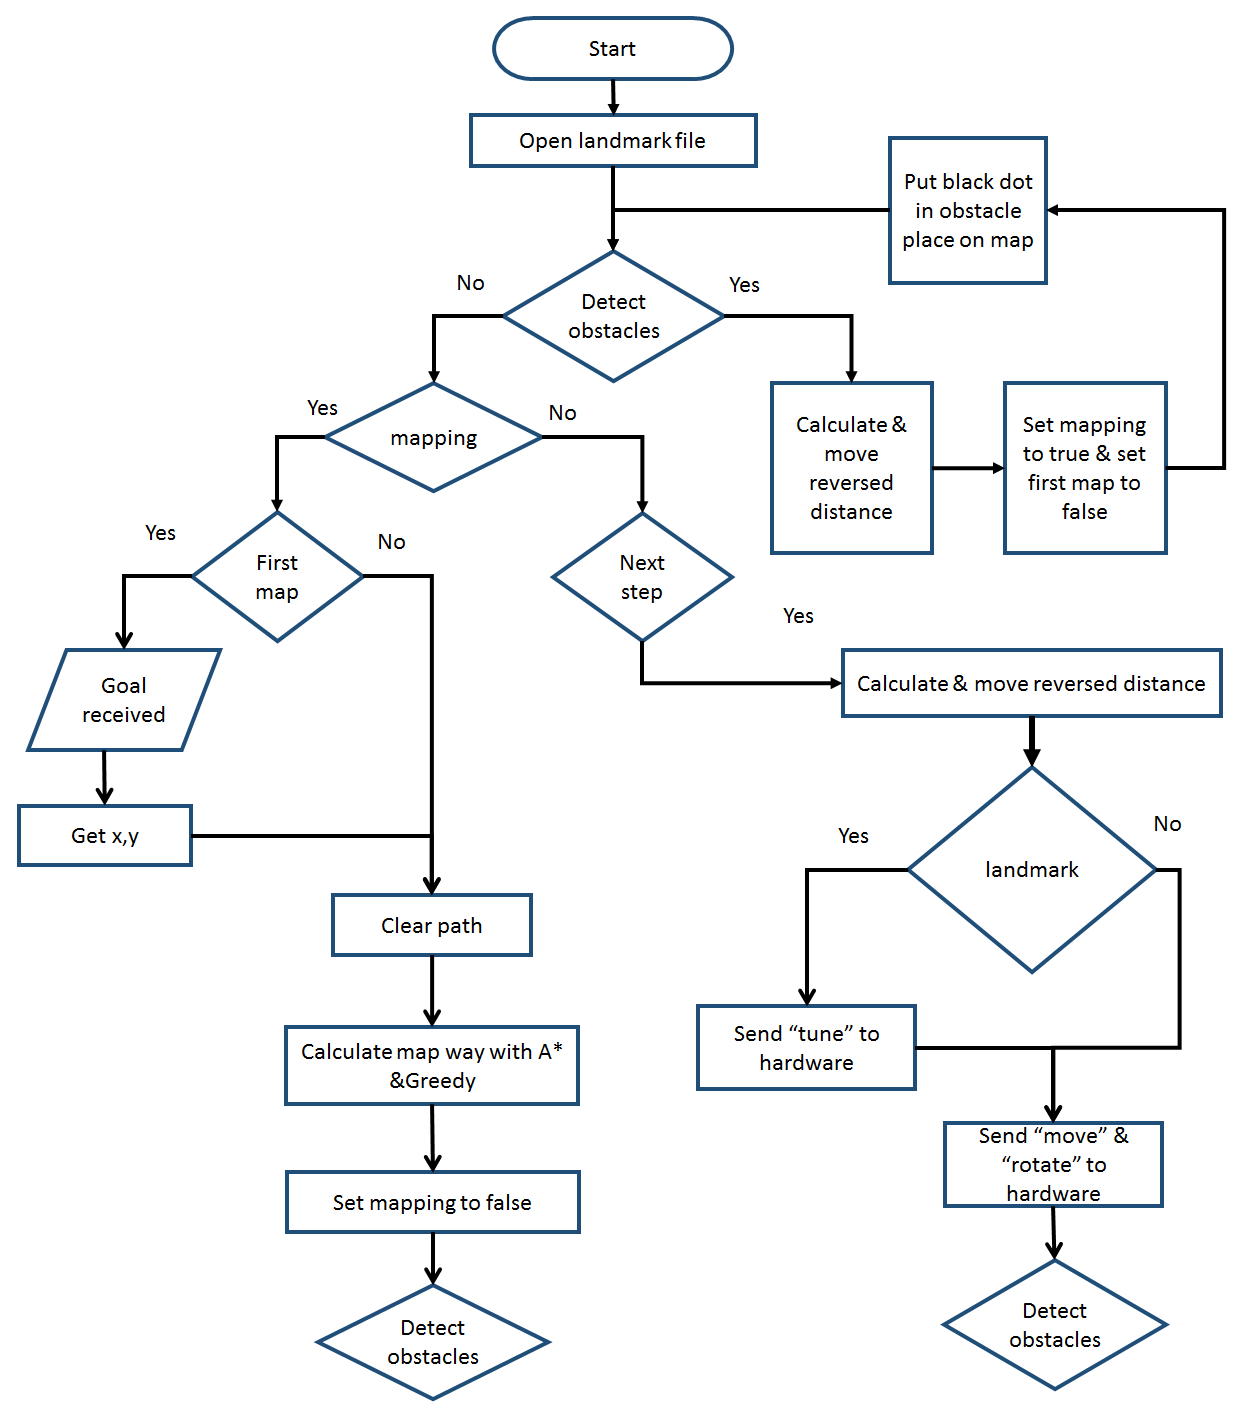
\includegraphics[width =1\textwidth]{Fig/mapping-flowchart.png}
	\caption{Flowchart of mapping process.}
	\label{fig:map-flowchart}
\end{figure}

\subsection{Mapping Example of indoor environment}
As we said first we use two kinds of search algorithm A* and GBFS. So, when the robot use them , as we show in this figure .. the map is build by colors from 0 to 255. 
We use three colors  , if a robot in 127 color so it use A* search and the 195 color is detection rejoin if the robot in it  should be ready to detect a land mark and the land mark is represented by 200 , otherwise the robot use greedy search , as this way we granted the robot always try to use greedy search to reduce the cost .

\begin{figure}[H]
	\centering
	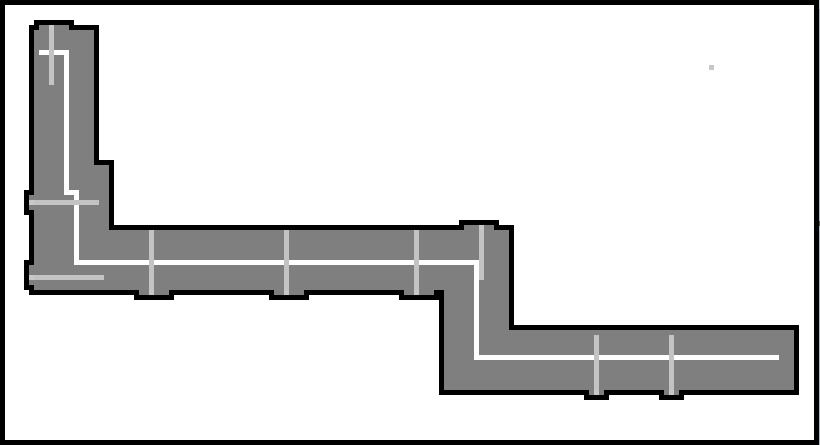
\includegraphics[width =.5\textwidth]{Fig/map-example.png}
	\caption{Map example represented in bitmap file.}
	\label{fig:map-example}
\end{figure}

\begin{figure}[H]
	\centering
	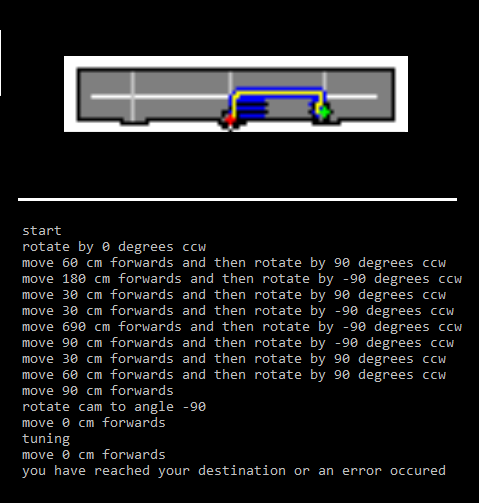
\includegraphics[width =.8\textwidth]{Fig/path-example.png}
	\caption{Path example and commands created from some source to destination in a trial map.}
	\label{fig:path-example}
\end{figure}

\newpage

\section{Computer Vision}
If robot is designed to blindly access the environment, its error rate will increase and its uses will be limited, So we used a Couple of Cameras with our robot for it to properly “see” the environment and better interact with it , we also used a library Called OpenCV which is – as the name implies – an Open source Computer Vision library , with methods used to process photos and extract info from them , we will use this library to help us locate our robots via landmarks , and detect and avoid obstacles (as a helping factor in addition to ultrasonic) , among other things.

\subsection{Landmark detection for Localization}
Our robot uses an offline map to navigate its environment , so it needs a landmark to use as a starting point , it may also use them as proof it has reached a specific point in the map and to compensate for errors , good , but how?\\

\noindent OpenCV is good with detecting circles , so we first chose our landmarks to be a thick circle with a number in it , when the robot is placed in a certain place , it spins around itself until it sees a landmark , then it goes and stands next to it , also when it knows (from the offline map) ,  that it is standing next to a landmark ,  it takes a photograph to confirm its location , the algorithm detects if there are two circle inside one another (the thick circle inner and outer perimeters) , then it confirms the results by cropping the outer circle and detecting the inner circle , the function returns the biggest thick circle in the scene and then recognizes it via OCR to determine which landmark it is , compare OCR results with landmark text it expects to find the best match.\\

\noindent This approach was not very good as circles get mis-recognized by the
Tesseract OCR engine we used to recognize which landmark it is, so we decided to detect rectangles instead of circles, and we made the landmarks to be white small rectangular cards (which will work fine with better results than circles as long as the door it’s sticked to is not white too) , and to solve the OCR problem further we used two OCR engines : Tesseract and OCRad , to get better results (these were the only two free OCR engines we could find).\\

\noindent Experimental result for landmark detection and recognition is shown in figure \ref{fig:landmark-result}.

\begin{figure}
	\centering
	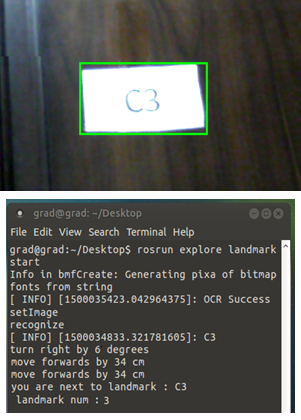
\includegraphics[width =0.8\textwidth]{Fig/landmark-result.png}
	\caption{Detection and recognition of landmark.}
	\label{fig:landmark-result}
\end{figure}

\newpage

\subsection{Using Computer Vision for obstacle avoiding}
Of Course an obvious question arises here , if we are already using Ultrasonic Sensors to detect obstacle , wouldn’t it be redundant to use Computer Vision as well ? Of course extra precautions never hurts , but there is another reason , Ultrasonic sensor only detects the obstacle if its normal to the sensor , otherwise the ultrasonic signal will reflect away from the surface and won’t be detected.\\

\noindent There are many ways to detect obstacles using computer vision , but each one has its pros and cons , we will discuss the methods we tried with our robot here.

\subsubsection{Canny Technique}
The technique depends on detecting the edges of the objects in the image , by blurring the image and using the canny transform , we get the edges of the objects in the image ,if the floor is not very rough it will have no edges and then it will be very simple to detect obstacles and walls!\\

\begin{itemize}
	\item Advantages:
	\begin{itemize}
		\item Easy to understand and implement 
		\item Super-Fast
		\item Gives decent results in simple situations
	\end{itemize}
	\item Disadvantages:
	\begin{itemize}
		\item Does not work when floor is rough or has different colors 
	\end{itemize}
\end{itemize}

\subsubsection{Floor Subtraction Technique}
The technique depends on subtracting the most significant blob near the bottom of the image , which is bound to be the floor , keeping only the obstacles and the walls , the robot finds the longest path it can walk in without hitting anything and turns left or right accordingly , yes , it’s as simple as that!

\begin{itemize}
	\item Advantages:
	\begin{itemize}
		\item Easy to understand and implement 
		\item Very Fast
		\item Gives decent results
		
	\end{itemize}
	\item Disadvantages:
	\begin{itemize}
		\item gets complicated (but solvable) when floor has different colors 
		\item The robots design obscures its view of the ground (not solvable)
		
	\end{itemize}
\end{itemize}

\subsubsection{Stereo BM/SGBM Techniques}
That’s how professionals do it ! BM/SGBM Stand for Block Matching / Semi Global Block Matching techniques , Both techniques are very similar , they both use two cameras as left eye and right eye , they both use a transform to find out which parts in the images are similar, they both return a grayscale map where near objects are brighter than far ones , this way we can detect obstacles as the near objects that are higher than a certain threshold from the floor , and find our way round them by finding the darkest part of the image and move towards it!
•	SGBM is more accurate than BM but it consumes much more time , so it’s a tradeoff between time and accuracy

\begin{itemize}
	\item Advantages:
	\begin{itemize}
		\item Most accurate and professional way to find obstacles
		\item Works on all kinds of floors
	\end{itemize}
	\item Disadvantages:
	\begin{itemize}
		\item Consumes large portions of processing power and memory
		\item Slower than other methods
	\end{itemize}
\end{itemize}

\subsubsection{Used Method}
We used SGBM while reducing the image size by 1/(8x8) of its original size to increase speed , the method uses threshold to determine whether there is something closer than a given distance and sends a remap command to the Mapping part if there is , it takes about half a second to process every frame so it should detect the obstacle when it’s half a second away.

\newpage

\section{Hardware Node and Modules Structure Tree}
In prior sections we always look at hardware as a black box. This view is sufficient when we want to describe the overall operation of the robot. But lets now take this part in some details to know how instructions are processed after being received from either mapping or computer vision node. \\
In the design stage of hard ware, One of the most important aspects taken into consideration is modularity of design. Each Part in the hardware structure has a unique role and a method by which this role can be triggered for execution. Another important style of design followed is assigning low level tasks to multiple separate modules rather than having a central unit responsible for the whole operation. This method of design saves a lot of resources in the master unit opening the way for other complicated operations to be performed faster. In the following sections we will talk first about the role of hardware ROS node and then go down at low level.

\subsection{Hardware ROS node}
As mentioned in figure \ref{fig:full-algorithm} the hardware node stands midway between both mapping and computer vision nodes. its main role is receiving instructions from other nodes, refining them and forwarding them to low-level modules to be performed by robot. This leads to two important results. First, the hardware ROS node is free of low-level operations which keeps its main role of regarding and communicating with other nodes. Second, low level modules save their processing capability for optimized motion and performance rather than being concerned with communication of multiple parts. 
\begin{figure}[H]
	\centering
	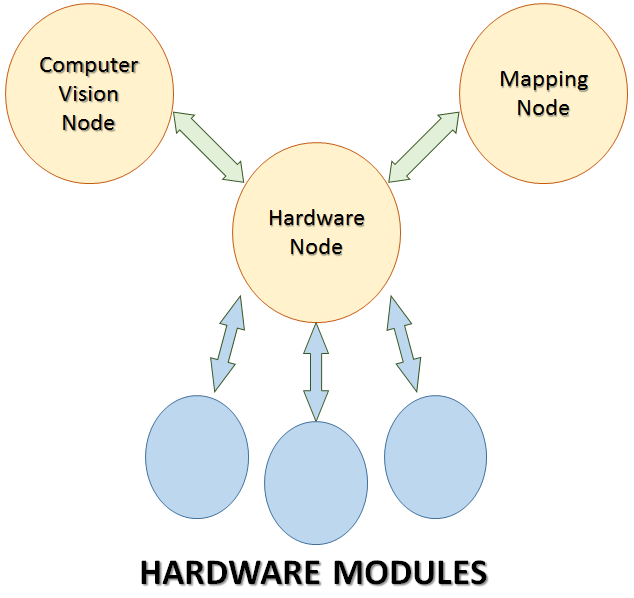
\includegraphics[width =0.45\textwidth]{Fig/hw-node.png}
	\caption{Hardware node standing midway between ROS nodes and hardware modules.}
	\label{fig:hw-node}
\end{figure}

\newpage

\subsection{Low-level Hardware Kits and Modules}
Here we reached to the stage of choosing the suitable kits and modules that can meet the needs of other nodes. In this case We must first encounter the whole instructions hardware may receive. These commands are as follow:
\begin{itemize}
	\item move straight some distance
	\item rotate robot some degrees
	\item set camera orientation
	\item measure distance between robot and any object around
	\item switch on flash light
	\item set motors speed
\end{itemize}
Each of these instructions has some requirements to be done. The modules we brought to fulfill these requirements can be encountered as follow:
\begin{center}
	\begin{tabular}{| c | c | c|}
		\hline
		Component & Function & Number of units \\
		\hline
		\hline
		Raspberry Pi R3 & Master Unit & 1\\
		\hline
		Arduino Nano Kits & processing units & 3\\
		\hline
		NodeMCU & micro controller with embedded WiFi module & 1\\
		\hline
		Motor driver & controlling motor speed and direction & 1\\
		\hline
		DC Motors & manipulators for robot motion & 4\\
		\hline
		Wheels & attached to motors & 4\\
		\hline
		Motor shaft encoder & counting revolutions of motor & 2\\
		\hline
		Compass Module & measuring heading angle & 1\\
		\hline
		Ultrasonic module & range finder & 4\\
		\hline
		Sharp IR sensor & range finder with longer distance span & 1\\
		\hline
		Camera & capturing the environment around & 2\\
		\hline
		Servo Motors & controlling camera orientation & 2\\
		\hline
		Lithium Battery & Power source for motors and Light & 1\\
		\hline
		Power bank 5V & Power source for Raspberry PI & 1\\
		\hline
		NiMH Battery 5V & Power source for Servo motors & 1\\
		\hline
	\end{tabular}
\end{center}

\noindent Components figures and data sheets are both included in appendix.

\newpage

\subsection{Hardware Tree Structure}
In this section we get closer to know how exactly project parts are connected to communicate. Also we will define the exact role for each part. As shown in figure \ref{fig:harware-structure} there are three sub nodes underlying the hardware node. Each one has sub-modules to control or communicate with. All these nodes are implemented on Arduino kits and this is a magnificent advantage for ROS as it provides libraries that enables us to implement ROS nodes on such kits.\cite{205} So, for each node it can publish and subscribe for message from the main hardware node on Raspberry Pi master. This enables us to have a single type of communication valid to use in all parts. We can identify the role of each node as follow:
\begin{itemize}
	\item \textbf{Manipulator Node:}\\
	This node is responsible for executing motion commands. The controller is implemented in this node. As we can see in figure \ref{fig:harware-structure} there three underlying parts, the motor driver, flash light and ultrasonic. You may wonder why ultrasonic is here in the manipulator node. This simply because we needed to summarize all parts that participate in the motion control in a single node to minimize the flow of communication message as possible. The motor driver has two tasks; sending speed signals to motors and combine the encoder pulses to the Arduino. More details about each module will be figured out in next sections.
	
	\item \textbf{Sensors Node:}\\
	Like the previous node, this one is implemented on an Arduino Nano kit and attached to it other sensors included in our project; Compass, Ultrasonic, IR range finder and servo motors that control the orientation of camera. One of the critical tasks this node is responsible for is regarding the front path of robot to give alarms if there is some obstacle. Another task is participating in estimation of robot orientation when rotation motion is performed. More details about each sensor and how we get use of its readings will be discussed in lated sections. 
	
	\item \textbf{Manual Controller Box:}\\
	This node is considered the main tool for adding a feature that the robot can be controlled remotely by man. Here in this node the main objective is giving user the ability to guide robot, change camera orientation and switching on/off flash light. This feature is so useful in exploration of new environments whose map is not available for autonomous motion. and it opens the way for adding on-line of such new environments.\\
	By determining the objective we can encounter the hardware units needed. So, for user-friendly controller we developed it using potentiometers and a switch connected to Arduino unit. And for publishing commands over the network a NodeMCU kit is used to implement a ROS publisher node on. 
	
	\begin{figure}[H]
		\centering
		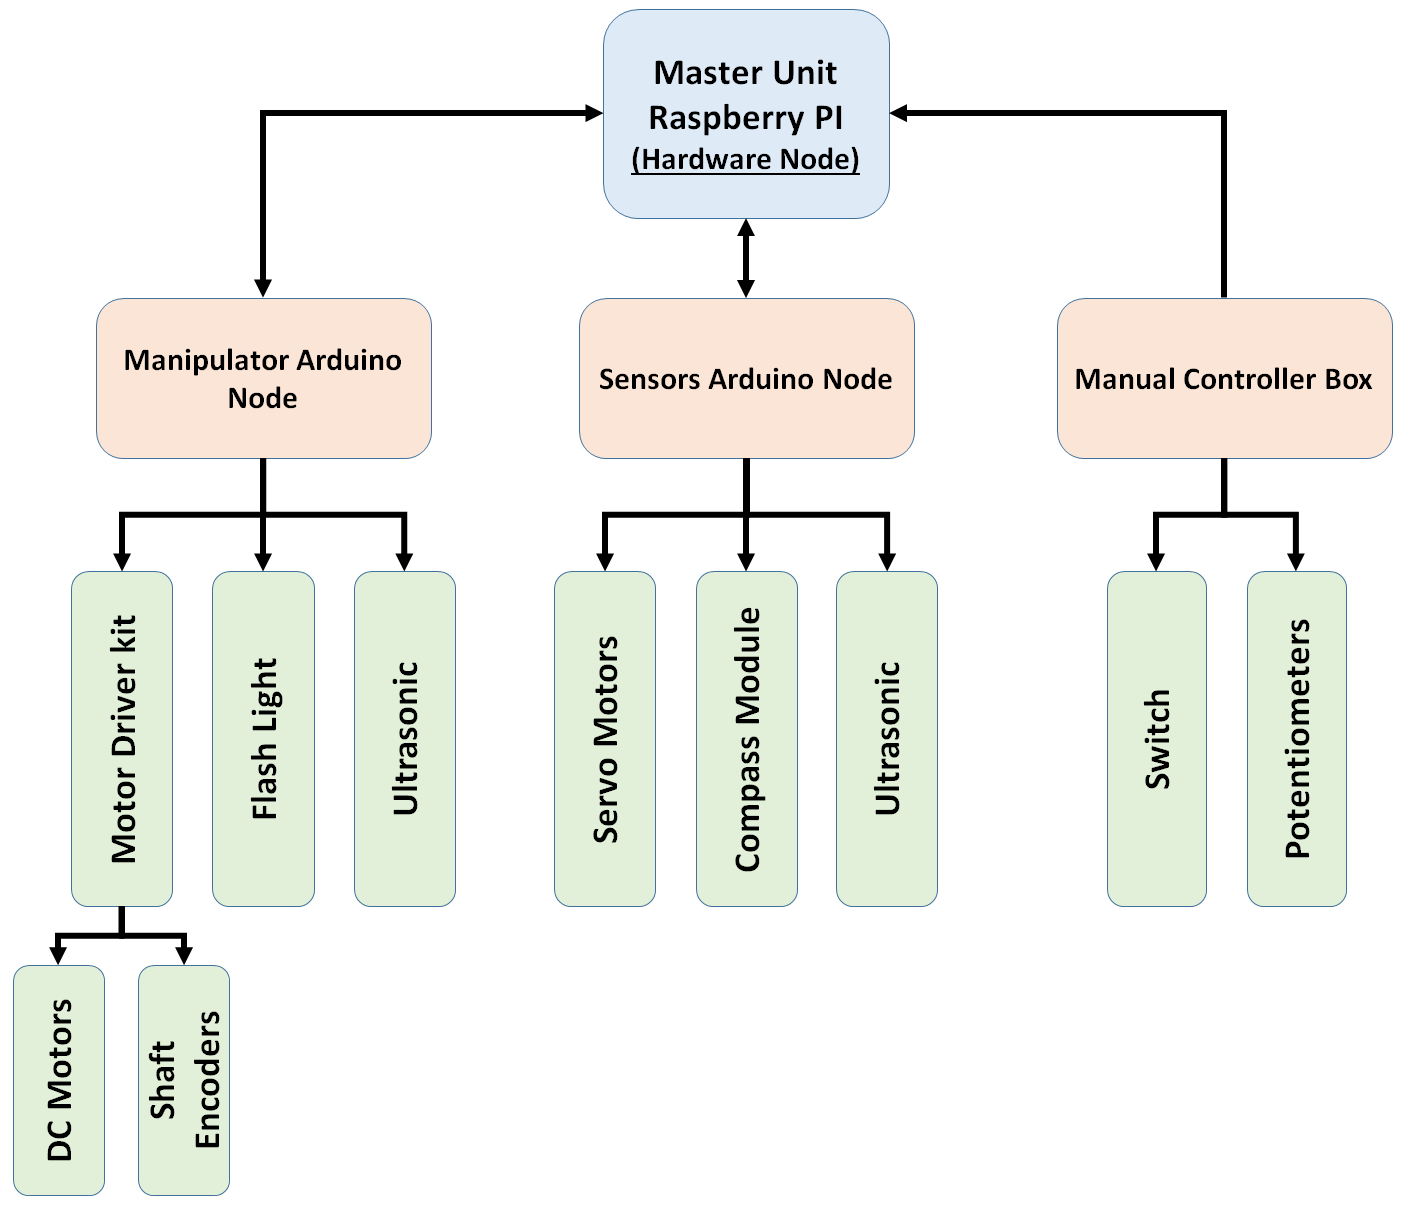
\includegraphics[width =0.9\textwidth]{Fig/hardware-structure.png}
		\caption{Hardware modules structure.}
		\label{fig:harware-structure}
	\end{figure}

	
\end{itemize}

\subsection{Electronics Involved in Project}
In this part we are to talk about electronics modules and components used in out project. For each components we will discuss its function, how it is operated, advantages, limitations and how we used it as a port of the full structure. Electronic components are to classified into four categories; processing units, sensors, passive components and power sources

\subsubsection{Processing Units}
\begin{itemize}
	\item \textbf{Raspberry PI R3}\\
	This part represents the master unit for the whole process. Its powerful processing capabilities opens the way complex processes that need much resources like CPU cycles or storage. One of these operations is the image processing and computer vision operated in out project. all the other parts are connected to Raspberry Pi by some way in a tree structure fashion. The operating system running on such unit is Ubuntu Mate 16.04 and we installed ROS platform base on it. We communicate and deal with this unit using SSH (Secure Shell) connection operated remotley from any other computer device.
	\begin{figure}[H]
		\centering
		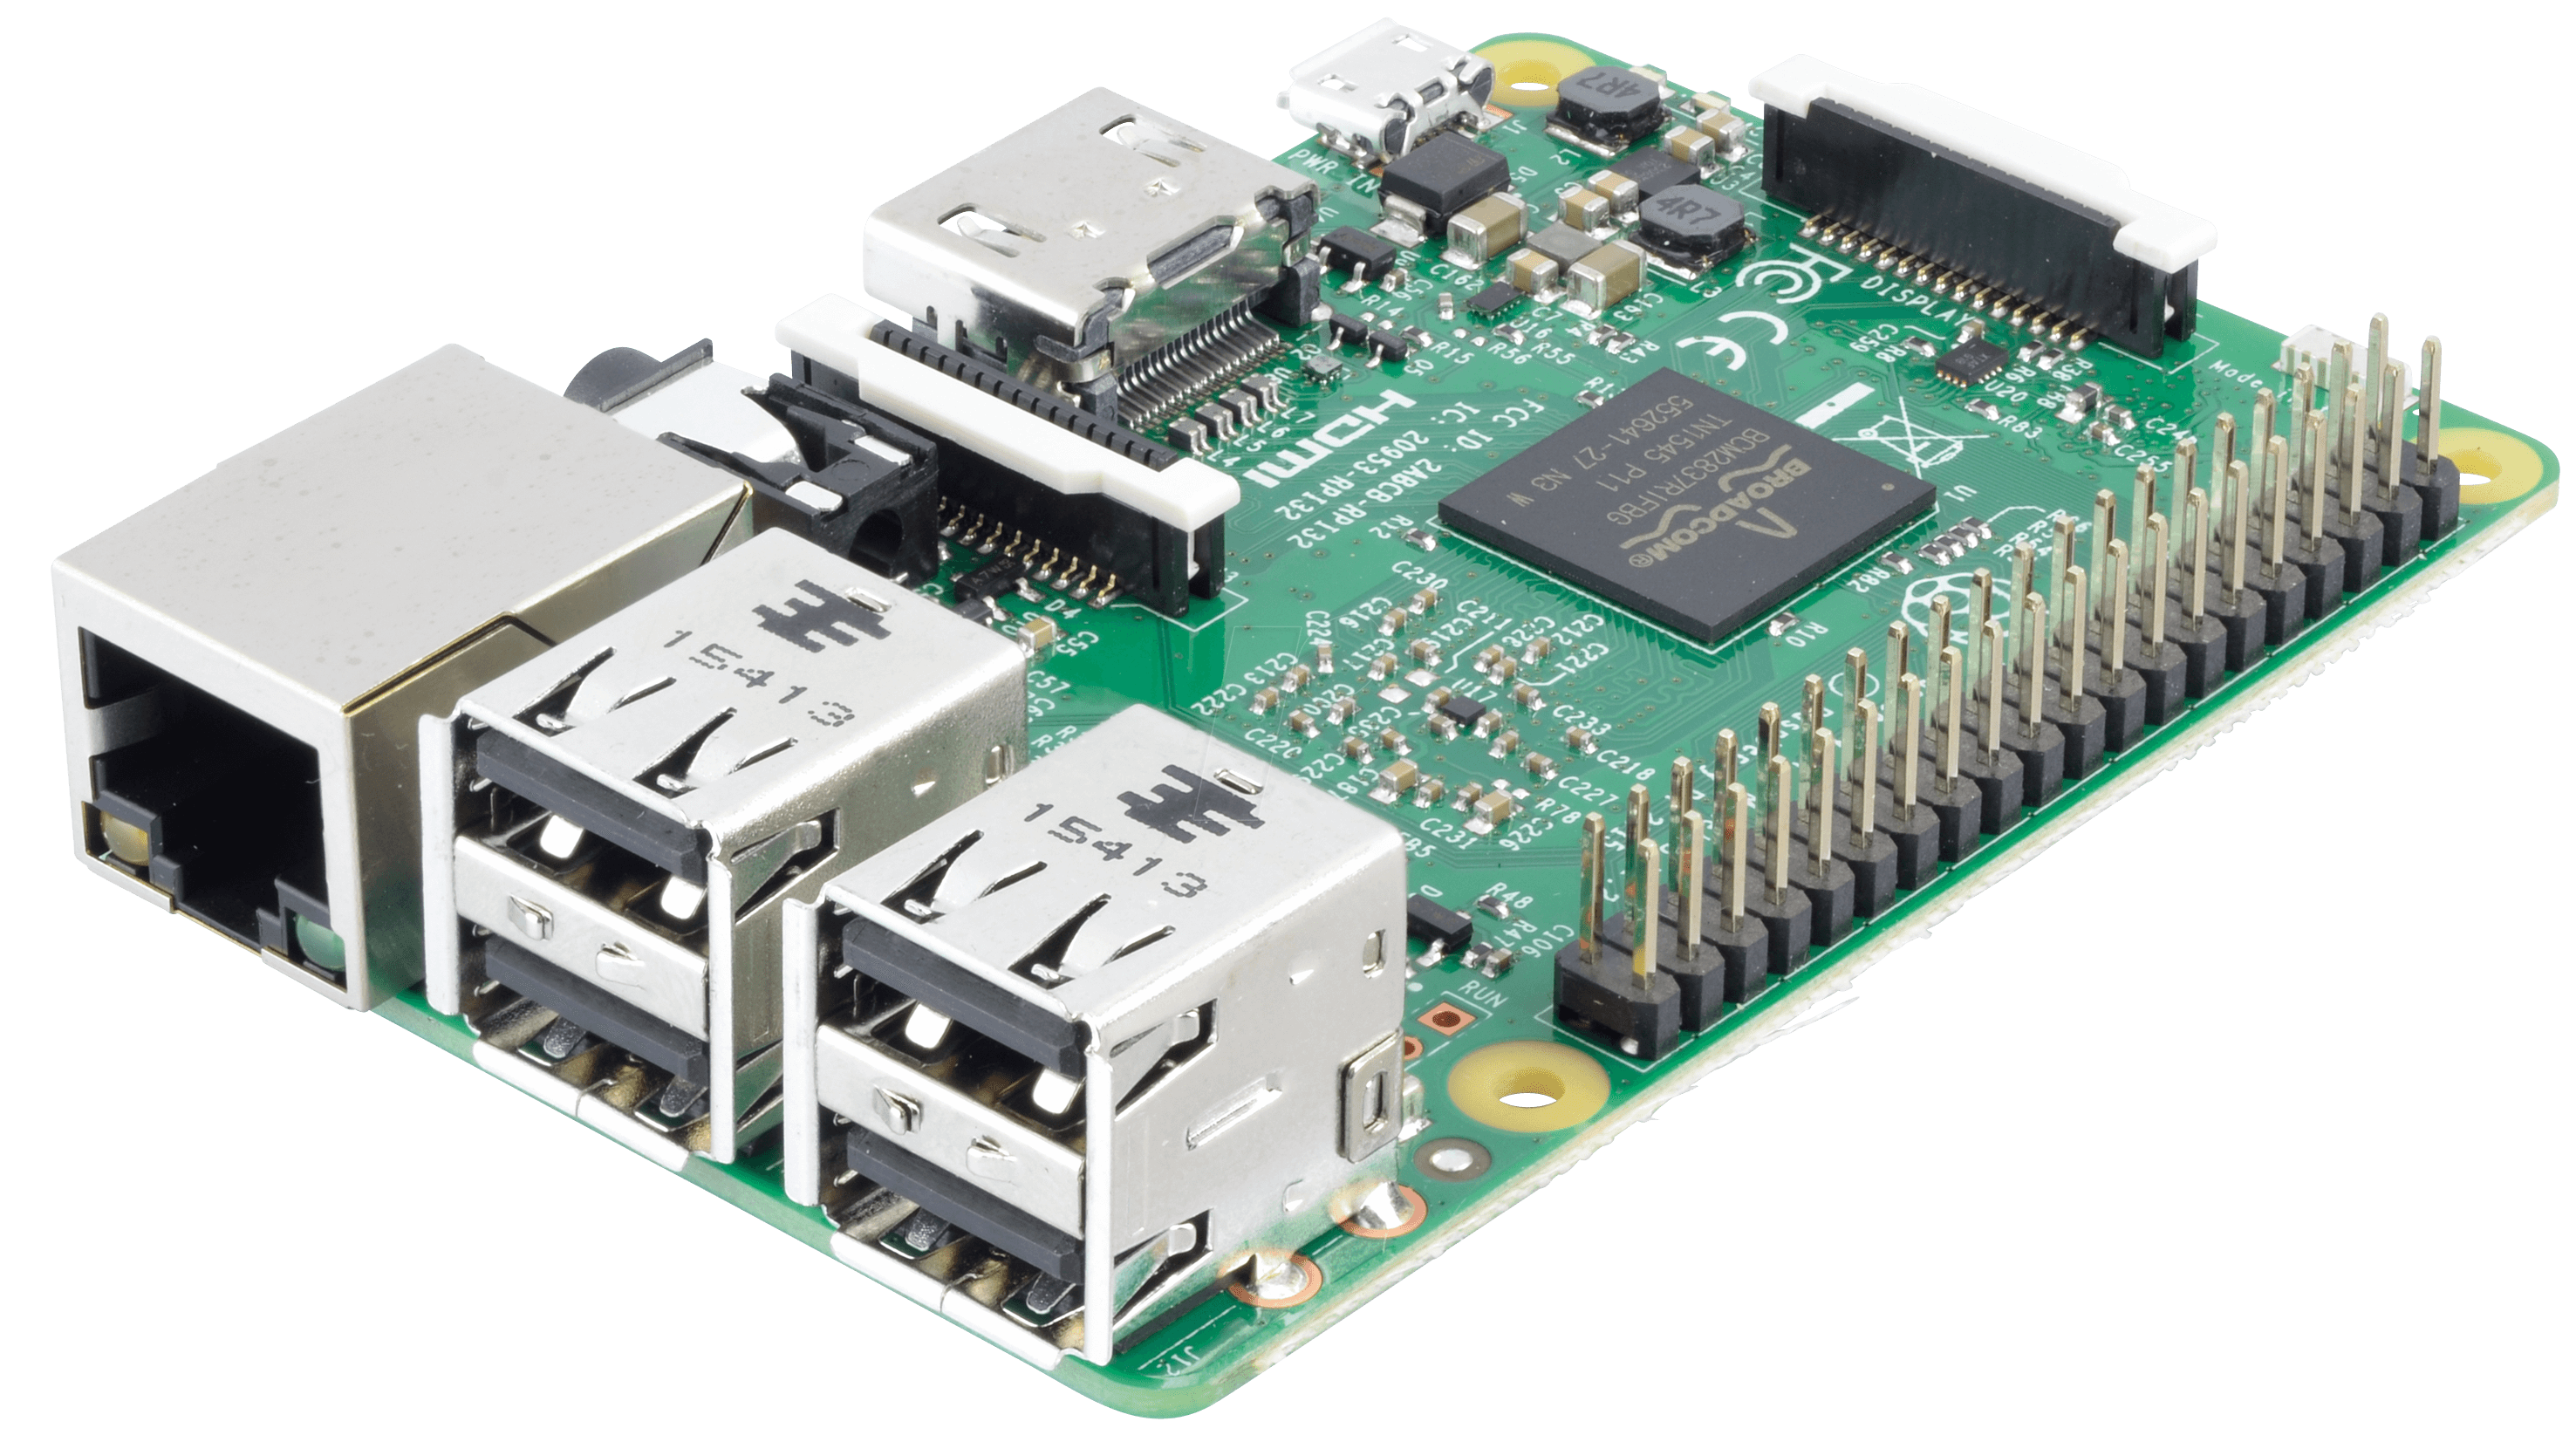
\includegraphics[width =0.6\textwidth]{Fig/Electronics/Raspberry.png}
		\caption{Raspberry Pi R3.}
		\label{fig:raspberry}
	\end{figure}

	\item \textbf{NodeMCU}\\
	This unit is a developed with integrated WiFi module. This helped us too much in the design of the manual controller box. We implemented a ROS node on it that publishes the instructions which can guide the robot and control camera orientation or flash light. This design and procedure will be explained in the software development section.
	We deal with this kit like an ordinary Arduino and program it using same Arduino IDE after installing some updates.
	
	\begin{figure}[H]
		\centering
		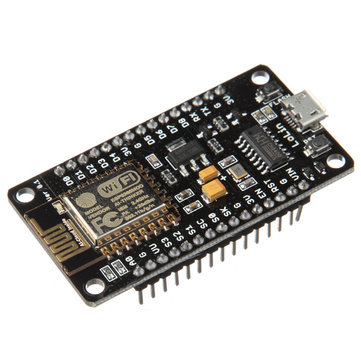
\includegraphics[width =0.4\textwidth]{Fig/Electronics/nodemcu.jpg}
		\caption{LoLin V3 NodeMcu}
		\label{fig:nodemcu}
	\end{figure}
	
	\item \textbf{Arduino Nano}\\
	This kit is limited but powerful processing unit that can be used in too many tasks and applications. Its small size, low cost and ease of use make it most common in many projects. In our project we used three kits of such type. First in the manipulator node that gets the motion instructions, run the controller and send output signals to motors. Second is used in Sensors node that have all sensors underlying it. This kits helped us too much in maintaining the modularity and integration of parts of our project.
	
	\begin{figure}[H]
		\centering
		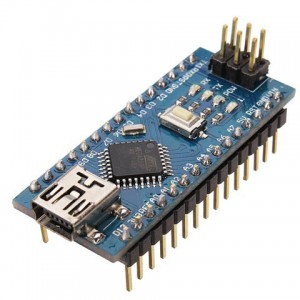
\includegraphics[width =0.3\textwidth]{Fig/Electronics/nano.jpg}
		\caption{Arduino nano kit}
		\label{fig:nano}
	\end{figure}

\end{itemize}

\subsubsection{Kits and Sensor modules}
\begin{itemize}
	\item \textbf{Motor Driver}\\
	There are a lot of modules having the function of controlling DC motors. Each has it own specs like max current, operating voltage and temperature. We find this kit is most suitable for our robot as it contains 4 channels for 4 dc motors. Moreover it requires just two pins to control both speed and direction of motors. It also have important features; current sensor and impeded logic circuitry for handling Encoder signals come from shaft encoder sensor.
	Its Electrical specs are 12V operating voltage and max current of 4.5A for each channel. These features and specs make it the best choice for our robot.
	
	
	\begin{figure}
		\centering
		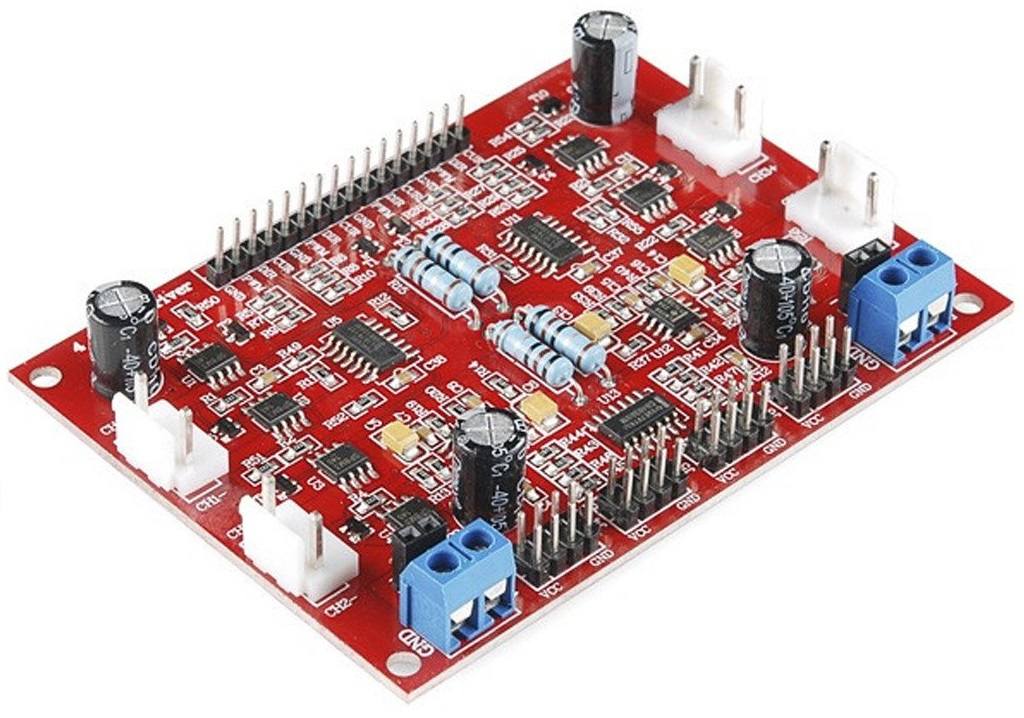
\includegraphics[width =0.5\textwidth]{Fig/Electronics/motor-driver.jpg}
		\caption{DC Motor Driver for Robot 4 channel}
		\label{fig:motor-driver}
	\end{figure}

	\item \textbf{Shaft Encoder}\\
	One of the most popular method of tracking the robot position is calculating the number of revolution each motor made. This way is called Odometry feedback. Each encoder has a property of number of pulses generated per revolution. This is an indication of how much distance change the robot can feel and encounter. The type we used in out project is 3 PPR. But our motor is geared with a gear head of ratio 1:30. That makes the exact value 90 pulses generated for each wheel revolution  Moreover, This Encoder has 2 channels each generates 3 pulses per revolution with phase shift 90 degrees. The logic circuitry in motor driver kit combines the two channels' pulses by an XOR gate resulting in an interrupt signal of 180 PPR. This gives a resolution of 0.21 cm per encoder interrupt pulse.\\ 
	But the most critical problem of this method of position estimation is that it may lead to fully wrong deviated measurements if the robot wheel slipped on the surface. There is no guarantee that the robot has already moved that distance without slipping. So, This drawback opens the way to think about how to make sure that the robot is actually moving not slipping.
	Figure \ref{fig:encoder-pulses} shows the two channel pulses and the resultant interrupt signal used by combining them through XOR Gate.\\
	
	\begin{figure}[H]
		\centering
		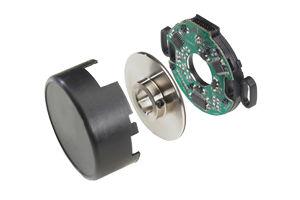
\includegraphics[width =0.6\textwidth]{Fig/Electronics/encoder.png}
		\caption{Motor shaft encoder 3PPR}
		\label{fig:encoder}
	\end{figure}
	
	\begin{figure}[H]
		\centering
		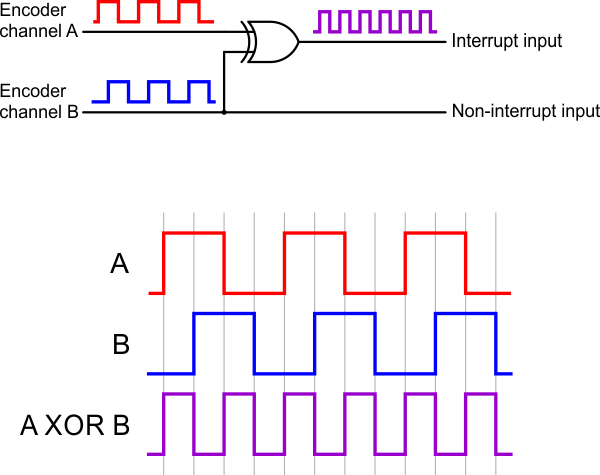
\includegraphics[width =0.4\textwidth]{Fig/Electronics/encoder-pulses.png}
		\caption{Quadrature encoder pulses explained}
		\label{fig:encoder-pulses}
	\end{figure}

	\item \textbf{Ultrasonic sensor}\\
		\begin{figure}[H]
		\centering
		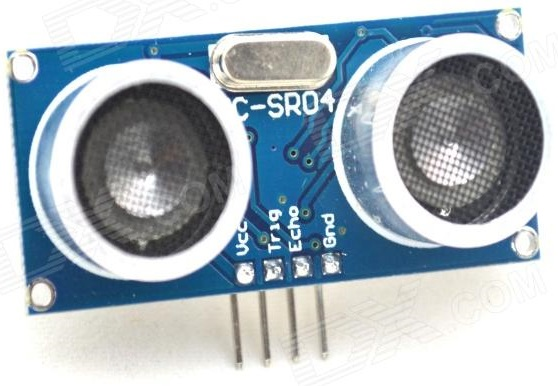
\includegraphics[width =0.4\textwidth]{Fig/Electronics/ultrasonic.jpg}
		\caption{Ultrasonic sensor}
		\label{fig:ultrasonic}
	\end{figure}
	This is a common sensor used for distance measurement between the sensor and the any object sitting in front of it. Its principle of operation depends upon sending an ultrasonic pulse and calculating the time passes until that signal echo come back and detected. The type we used has an operating range 1:300 cm. But there are many problems occur when using this sensor. These problems can be encountered as follow:
	\begin{itemize}
		\item accuracy of reading becomes bad while the measured distance increases.
		\item the procedure of measurement depending upon waiting until the signal comes back. This makes the processing unit idle and causes synchronization problems with other electronic modules running on the same micro-controller
		\item the sensor is not guaranteed to get a reading as the signal may be absorbed by some obstacle materials or reflected far away on inclined surface of the obstacle.  
	\end{itemize} 

	
	\item \textbf{Compass Module}\\
	This sensor make use of measuring magnetic field of earth to get the heading angle(the angle between X axis of module and North directing ), We paid this sensor much intention at first steps of work because it gives an absolute angle of robot heading which can be combined with encoder information about the displacement of robot to get a full estimation of robot location from the start point. But during our work we faced many problems that made us can not depend on its reading for estimation of robot position or heading. \\
	\begin{figure}[H]
		\centering
		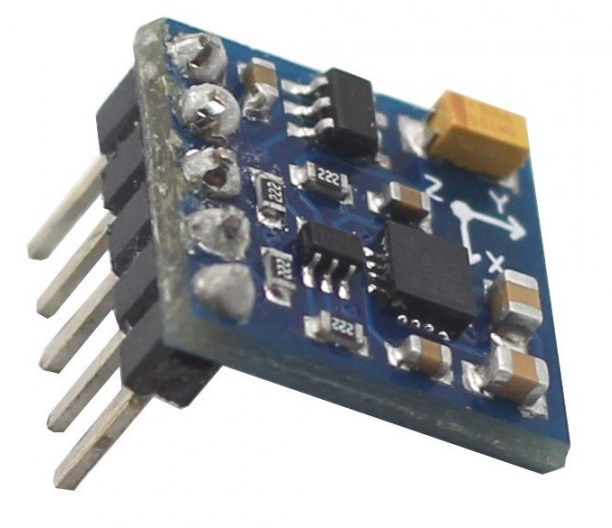
\includegraphics[width =0.3\textwidth]{Fig/Electronics/compass.jpg}
		\caption{compass module HMC5883L}
		\label{fig:compass}
	\end{figure}
	The worst problem associated with this module is that it is affected by any magnetic field around it. This is a big problem because indoor navigation makes the robot among too many electrical devices that generate different magnetic field patterns and so different effects on compass reading. Compass reading may encounter a scaling problem, dc shift or combination of them.
	To visualize this problem, we plot te compass readings while rotating it, the pattern we get is shown in figure \ref{fig:compass-sh}.\\
	\begin{figure}[H]
		\centering
		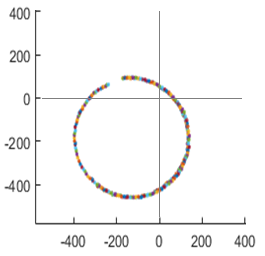
\includegraphics[width =0.4\textwidth]{Fig/compass-sh.png}
		\caption{Showing the shifting problem in compass readings}
		\label{fig:compass-sh}
	\end{figure}
	About the sensitivity we took a reading pattern while rotating the compass and repeated the process at same place but a mobile phone was put at distance of 20 cm away from the module. the pattern was changed in both shift ans scale values. This result is shown in figure \ref{fig:compass-diff-sh}
		\begin{figure}[H]
		\centering
		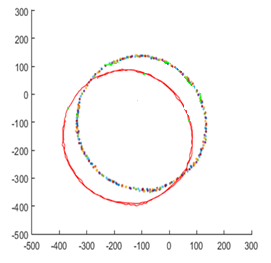
\includegraphics[width =0.4\textwidth]{Fig/compass-diff-shift.png}
		\caption{Showing the shifting problem in compass readings}
		\label{fig:compass-diff-sh}
	\end{figure}
	
	\item \textbf{Accelerometer and Gyroscope}\\
	\begin{figure}[H]
		\centering
		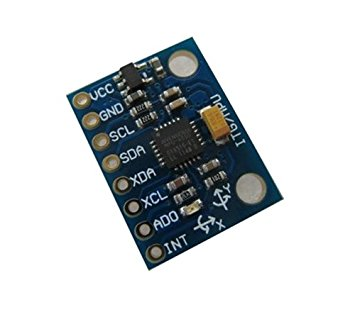
\includegraphics[width =0.4\textwidth]{Fig/Electronics/mpu.jpg}
		\caption{MPU6050 Accelerometer and Gyroscope}
		\label{fig:mpu}
	\end{figure}
		
	\item \textbf{IR Range Finder}\\
	\begin{figure}[H]
		\centering
		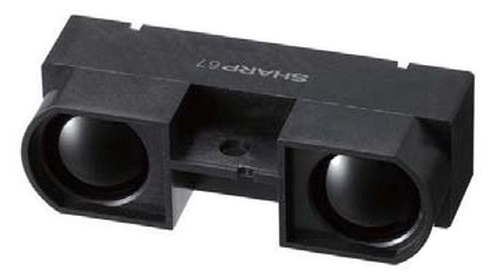
\includegraphics[width =0.4\textwidth]{Fig/Electronics/ir.jpg}
		\caption{IR sharp sensor}
		\label{fig:ir}
	\end{figure}
\end{itemize}

\subsubsection{Power Sources}
\begin{itemize}

	\item \textbf{Power Bank 5V}\\
	\begin{figure}[H]
		\centering
		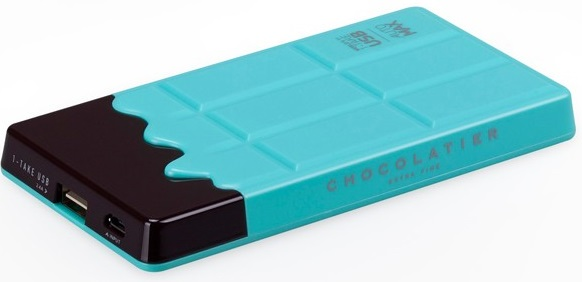
\includegraphics[width =0.5\textwidth]{Fig/Electronics/power-bank.jpg}
		\caption{Power Bank "Rechargeable Battery Pack" 7000mAh}
		\label{fig:powerbank}
	\end{figure}

	\item \textbf{Lithium-ion 12V Battery}\\
	\begin{figure}[H]
		\centering
		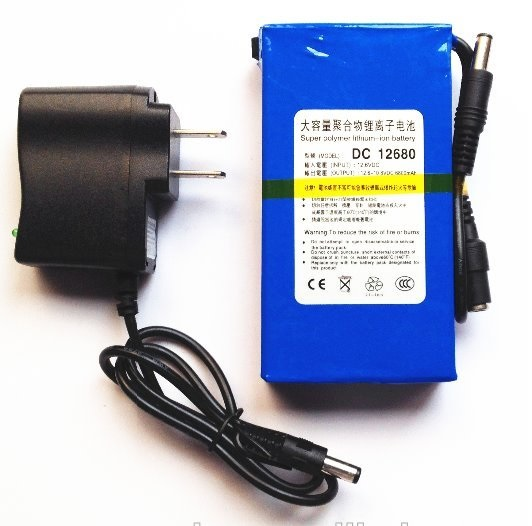
\includegraphics[width =0.5\textwidth]{Fig/Electronics/bat12.jpg}
		\caption{Lithium-ion Super Rechargeable Battery Pack (12V, 7000mAh)}
		\label{fig:bat12}
	\end{figure}
	
		\item \textbf{NiMH 5V Battery}\\
	\begin{figure}[H]
		\centering
		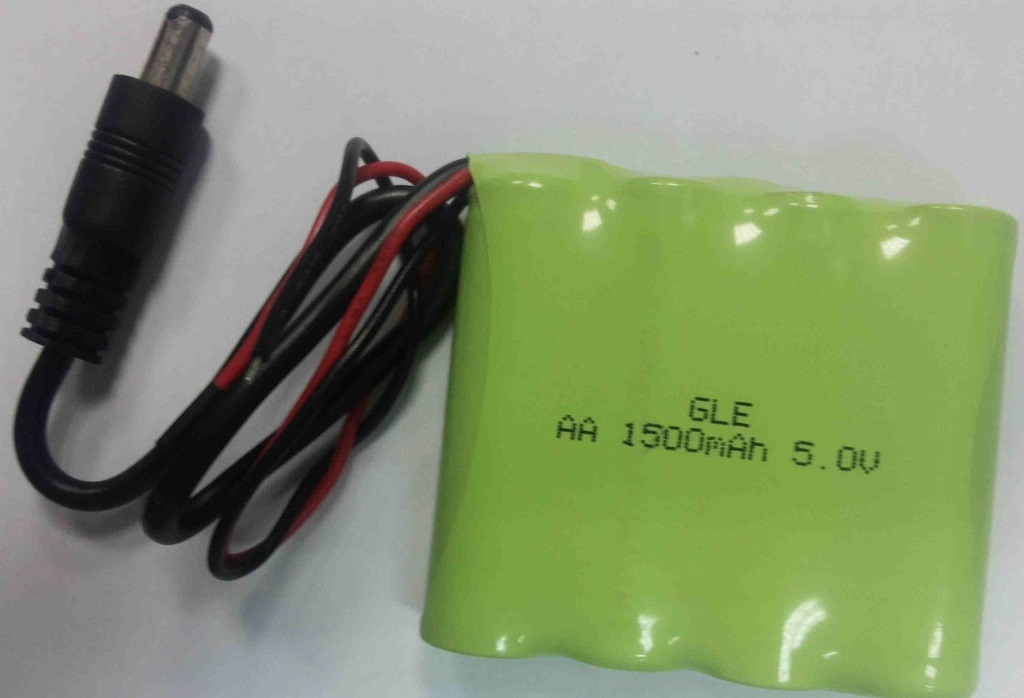
\includegraphics[width =0.5\textwidth]{Fig/Electronics/bat5.jpg}
		\caption{NiMH Rechargeable Battery (5V-1500mAh)}
		\label{fig:bat5}
	\end{figure}
	
\end{itemize}

\subsubsection{Passive Components}
\begin{itemize}
	\item \textbf{Potentiometer}\\
	\begin{figure}[H]
		\centering
		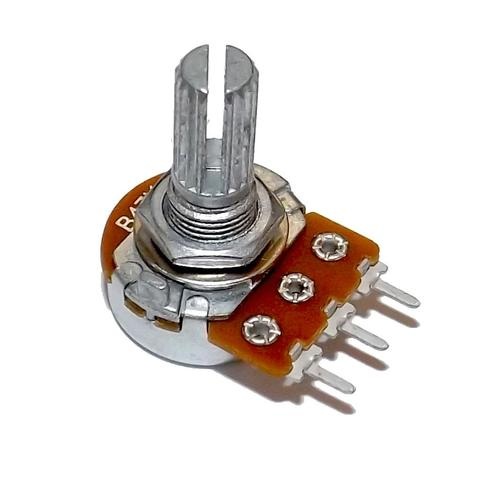
\includegraphics[width =0.5\textwidth]{Fig/Electronics/pot.jpg}
		\caption{Potentiometer 50 Kohm }
		\label{fig:pot}
	\end{figure}

	\item \textbf{LEDs}\\
	\begin{figure}[H]
		\centering
		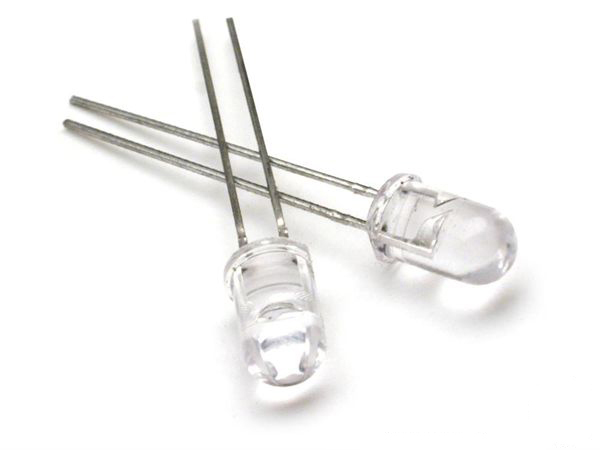
\includegraphics[width =0.5\textwidth]{Fig/Electronics/LED.jpg}
		\caption{White LEDs 5 mm 3V}
		\label{fig:led}
	\end{figure}

\end{itemize}

\newpage

\section{Software Implementation of Micro-Controller nodes}

\subsection{WiFi Reamot Controller}

\subsection{Manipulator Node}

\subsection{Sensors Node}

\newpage

\section{Mechanical Design}
In this section we are about to take a close look on the design procedure of robot hardware both mechanical and electrical. The design stage of any application depends on the tasks and requirements it is supposed to fulfill. So, we will talk about functional requirements of project and how we select components to best suit them. Design engineers are usually constrained by one or more of these 5 concerns; time, money, knowledge, power and weight. So, there is no absolute good choice but we try to select the best one that meets the requirements and follow constraints. \cite{203} Then we will get a brief view on frame design, materials used and how manufacturing operation done. After that we will get closer to the low level control and talk about electronic modules and sensors used, function, advantages and disadvantages of each. Finally we reach the controller design; how it was implemented, tuned and tested.  

\subsection{Choosing Suitable DC Motor  \cite{203}}
In this project we introduce a robot for indoor navigation. So, in this case low speed is acceptable but at the same time it must be powerful enough for carrying and transporting most of parts we deal with at home or office. The requirements of robot were selected to be as follow:

\begin{itemize}
	\item \textbf{Functional Requirements:}
	\\ DC Gear head motor capable of accelerating a 20 Kg, four-wheel drive robot with wheel diameter of 6.5 cm at a rate of 1 ${m/s^2}$. Top speed required will be around 0.75 m/s. This speed is suitable as it reasonably approachs human walking speed.
	\item \textbf{Design Parameters:}
	\\Supplied Voltage = 12 V, Motor size limited to an overall diameter of approximately 4 cm and an overall length of not more than 10 cm (Less than robot frame width).
\end{itemize}
Here is the calculation steps based on the lecture notes referenced in section title:
\begin{itemize}
	\item \textbf{Step One: Calculating Required Torque and rpm:}
	\begin{itemize}
		\item \textbf{Required Torque:} \\
		${Force = Mass \times Acceleration}$\\
		${F_{total} = ma = 20 kg \times 1 m/s^2 = 20 N}$\\
		${F_w = F_{total} \div NumberOfWheels = 20 \div 4 = 5N }$\\
		${\tau = F d = F_w \times WheelRadius = 5 N \times 0.065 m = 0.325 Nm}$\\
		
		\newpage
		
		\item \textbf{Required rpm:}\\
		${Wheel Circumference = C_w = \pi D = 3.142 \times 0.13 m = 0.408m}$\\
		${Speed = RPS \times C_w}$\\
		${RPS = Speed \div C_w = 0.75 \div 0.408m = 1.838 rps = 110.294 rpm}$\\
		
	\end{itemize}
	
	\item \textbf{Step Two: Motor Selection to Meet the Requirements}\\
	After searching available electronics stores we got the most suitable motor for our project. Its model name is SG-555123000-30K shown in figure . From the data sheet provided for it find the following specs:\cite{204}
	\begin{itemize}
		\item Rated Voltage : 12 V
		\item No load Speed : 100 rpm
		\item Load torque speed : 73 rpm
		\item Torque : 0.34 Nm
	\end{itemize}
	By these specs we can conclude that robot features became as follow:
	\begin{itemize}
		\item ${Full  load  speed = rpm \times C_w \div 60 = 73 \times 0.408 \div 60 = 0.4964 m/s}$
		\item ${Pay load = \frac{ \tau_w \times 4}{ R_w \times a} = \frac{0.34 \times 4}{0.065 * 1} = 20.923 kg}$
		
	\end{itemize}
\end{itemize}

This is still acceptable speed because the robot is not supposed to work in full load all time. Moreover the speed of about 0.5 m/s is suitable also for indoor navigation purposes.

\begin{figure}[H]
	\centering
	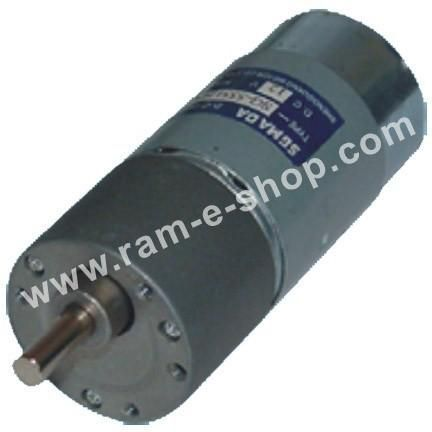
\includegraphics[width =0.35\textwidth]{Fig/dc-motor.jpg}
	\caption{DC motor SG-555123000-30K selected for driving the robot.}
	\label{fig:dc-motor}
\end{figure}



\newpage

\subsection{Robot Dimensions and Design Considerations}
\begin{figure}[H]
	\centering
	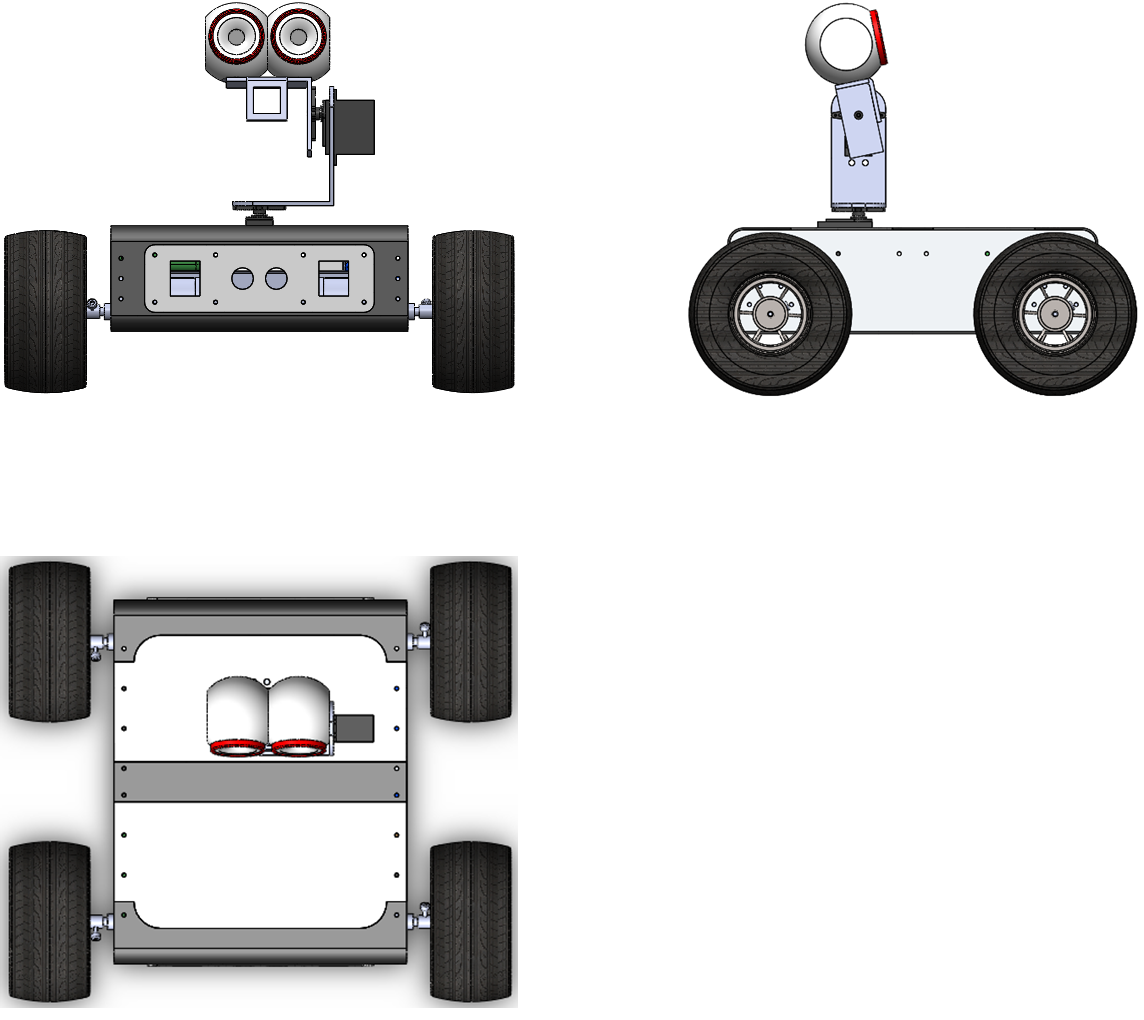
\includegraphics[width =0.8\textwidth]{Fig/solid/solid-planes.png}
	\caption{Front, side and top planes for assembly of robot frame}
	\label{fig:frame-planes}
\end{figure}

\begin{figure}[H]
	\centering
	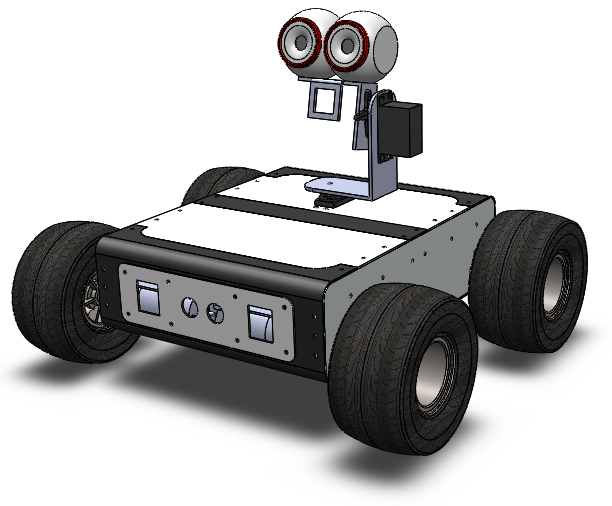
\includegraphics[width =0.4\textwidth]{Fig/Introduction.png}
	\caption{3D Real view of robot frame}
\end{figure}

%talk about old design
%aluminium design

\subsection{Mechanical Parts}
\begin{figure}[H]
	\centering
	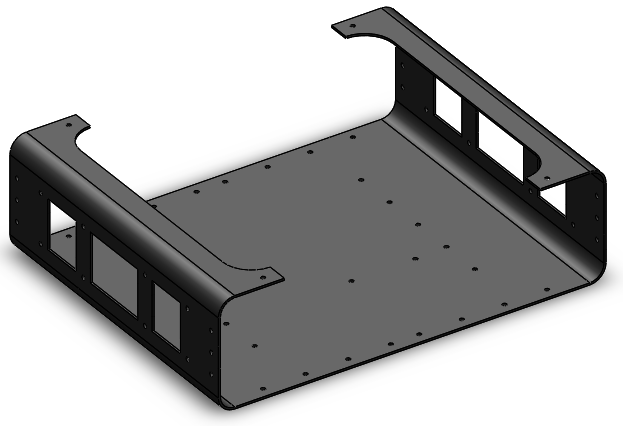
\includegraphics[width =0.8\textwidth]{Fig/solid/frame-3d.png}
	\caption{Aluminum Base frame}
\end{figure}

\begin{figure}[H]
	\centering
	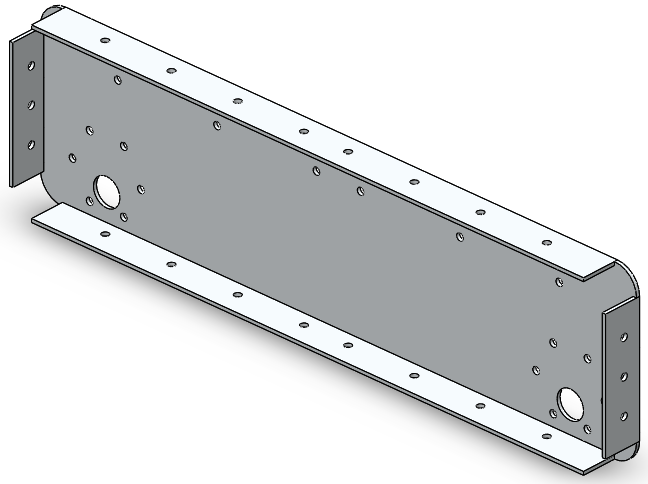
\includegraphics[width =0.6\textwidth]{Fig/solid/side-frame.png}
	\caption{Side frame}
\end{figure}

\begin{figure}[H]
	\centering
	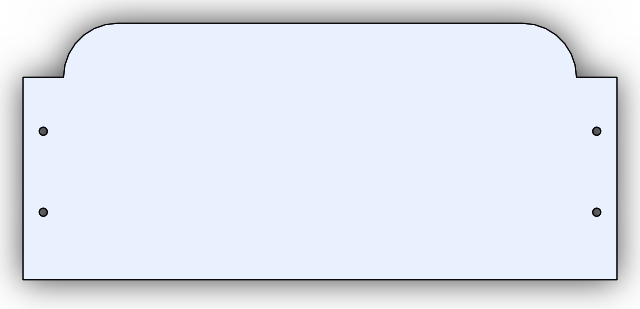
\includegraphics[width =0.8\textwidth]{Fig/solid/top-front-cover.png}
	\caption{Top front cover}
\end{figure}

\begin{figure}[H]
	\centering
	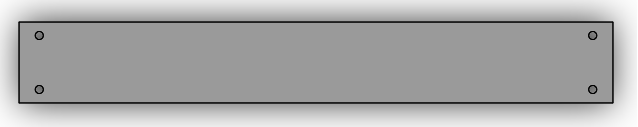
\includegraphics[width =0.8\textwidth]{Fig/solid/mid-part.png}
	\caption{Top mid link}
\end{figure}

\begin{figure}[H]
	\centering
	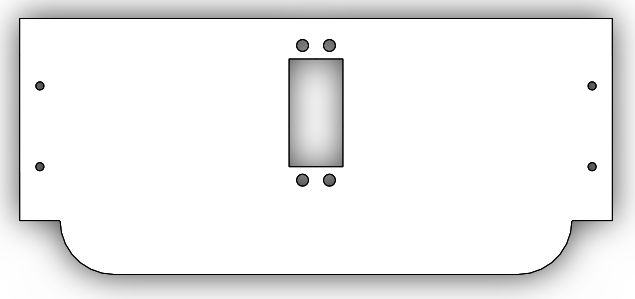
\includegraphics[width =0.8\textwidth]{Fig/solid/top-back-cover.png}
	\caption{Top back cover}
\end{figure}




\begin{figure}[H]
	\centering
	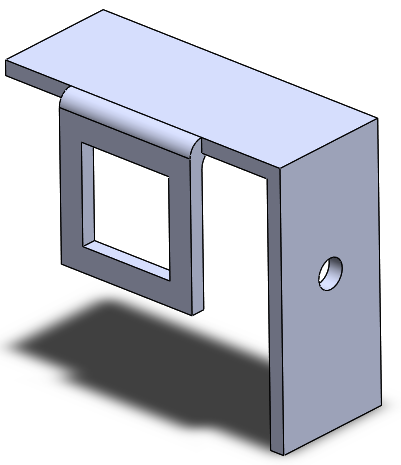
\includegraphics[width =0.5\textwidth]{Fig/solid/cam-holder-2.png}
	\caption{Upper Link of Camera Holder}
\end{figure}

\begin{figure}[H]
	\centering
	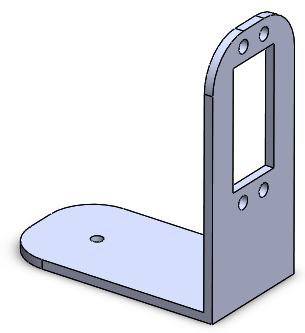
\includegraphics[width =0.5\textwidth]{Fig/solid/cam-holder-1.png}
	\caption{lower Link of Camera Holder}
\end{figure}


\begin{figure}[H]
	\centering
	\includegraphics[width =0.8\textwidth]{Fig/solid/Motor-cover.png}
	\caption{DC motors Cover}
\end{figure}

\newpage
\appendix

\newpage
 
\bibliographystyle{abbrv}
\bibliography{final}

\end{document}

